\documentclass[12pt,]{book}
\usepackage{lmodern}
\usepackage{amssymb,amsmath}
\usepackage{ifxetex,ifluatex}
\usepackage{fixltx2e} % provides \textsubscript
\ifnum 0\ifxetex 1\fi\ifluatex 1\fi=0 % if pdftex
  \usepackage[T1]{fontenc}
  \usepackage[utf8]{inputenc}
\else % if luatex or xelatex
  \ifxetex
    \usepackage{mathspec}
  \else
    \usepackage{fontspec}
  \fi
  \defaultfontfeatures{Ligatures=TeX,Scale=MatchLowercase}
\fi
% use upquote if available, for straight quotes in verbatim environments
\IfFileExists{upquote.sty}{\usepackage{upquote}}{}
% use microtype if available
\IfFileExists{microtype.sty}{%
\usepackage{microtype}
\UseMicrotypeSet[protrusion]{basicmath} % disable protrusion for tt fonts
}{}
\usepackage[margin=1in]{geometry}
\usepackage{hyperref}
\hypersetup{unicode=true,
            pdftitle={A Guide to Implementing Nutrition and Food Security Surveys},
            pdfauthor={Valid International},
            pdfborder={0 0 0},
            breaklinks=true}
\urlstyle{same}  % don't use monospace font for urls
\usepackage{natbib}
\bibliographystyle{apalike}
\usepackage{longtable,booktabs}
\usepackage{graphicx,grffile}
\makeatletter
\def\maxwidth{\ifdim\Gin@nat@width>\linewidth\linewidth\else\Gin@nat@width\fi}
\def\maxheight{\ifdim\Gin@nat@height>\textheight\textheight\else\Gin@nat@height\fi}
\makeatother
% Scale images if necessary, so that they will not overflow the page
% margins by default, and it is still possible to overwrite the defaults
% using explicit options in \includegraphics[width, height, ...]{}
\setkeys{Gin}{width=\maxwidth,height=\maxheight,keepaspectratio}
\IfFileExists{parskip.sty}{%
\usepackage{parskip}
}{% else
\setlength{\parindent}{0pt}
\setlength{\parskip}{6pt plus 2pt minus 1pt}
}
\setlength{\emergencystretch}{3em}  % prevent overfull lines
\providecommand{\tightlist}{%
  \setlength{\itemsep}{0pt}\setlength{\parskip}{0pt}}
\setcounter{secnumdepth}{5}
% Redefines (sub)paragraphs to behave more like sections
\ifx\paragraph\undefined\else
\let\oldparagraph\paragraph
\renewcommand{\paragraph}[1]{\oldparagraph{#1}\mbox{}}
\fi
\ifx\subparagraph\undefined\else
\let\oldsubparagraph\subparagraph
\renewcommand{\subparagraph}[1]{\oldsubparagraph{#1}\mbox{}}
\fi

%%% Use protect on footnotes to avoid problems with footnotes in titles
\let\rmarkdownfootnote\footnote%
\def\footnote{\protect\rmarkdownfootnote}

%%% Change title format to be more compact
\usepackage{titling}

% Create subtitle command for use in maketitle
\newcommand{\subtitle}[1]{
  \posttitle{
    \begin{center}\large#1\end{center}
    }
}

\setlength{\droptitle}{-2em}
  \title{A Guide to Implementing Nutrition and Food Security Surveys}
  \pretitle{\vspace{\droptitle}\centering\huge}
  \posttitle{\par}
  \author{Valid International}
  \preauthor{\centering\large\emph}
  \postauthor{\par}
  \predate{\centering\large\emph}
  \postdate{\par}
  \date{05/03/2018}

\usepackage{booktabs}
\usepackage{color}
\usepackage{tcolorbox}
\graphicspath{ {images/} }

\newenvironment{rmdremind}
  {\begin{tcolorbox}[width=\textwidth, 
                     colback = {white}, 
                     title = {\textbf{Remember}}, 
                     colbacktitle = lightgray,
                     coltitle = black]
  \begin{includegraphics}[scale = 1]{remind.png}
  \begin{itemize}}
  {\end{itemize}
  \end{includegraphics}
  \end{tcolorbox}}

\newenvironment{rmdnote}
  {\begin{tcolorbox}[width=\textwidth, 
                     colback = {white}, 
                     title = {\textbf{Note}}, 
                     colbacktitle = lightgray,
                     coltitle = black]
  \begin{includegraphics}[scale = 1]{pencil.png}}
  {\end{includegraphics}
  \end{tcolorbox}}
  
\newenvironment{rmdinfo}
  {\begin{tcolorbox}[width=\textwidth, 
                     colback = {white}, 
                     title = {\textbf{Info}}, 
                     colbacktitle = lightgray,
                     coltitle = black]
  \begin{includegraphics}[scale = 1]{info.png}}
  {\end{includegraphics}
  \end{tcolorbox}}  
  
\newenvironment{rmdwarning}
  {\begin{tcolorbox}[width=\textwidth, 
                     colback = {white}, 
                     title = {\textbf{Warning}}, 
                     colbacktitle = lightgray,
                     coltitle = black]
  \begin{includegraphics}[scale = 1]{warning.png}}
  {\end{includegraphics}
  \end{tcolorbox}}

\newenvironment{rmddownload}
  {\begin{tcolorbox}[width=\textwidth, 
                     colback = {white}, 
                     title = {\textbf{Download}}, 
                     colbacktitle = lightgray,
                     coltitle = black]
  \begin{includegraphics}[scale = 1]{download.png}}
  {\end{includegraphics}
  \end{tcolorbox}}

\usepackage{amsthm}
\newtheorem{theorem}{Theorem}[chapter]
\newtheorem{lemma}{Lemma}[chapter]
\theoremstyle{definition}
\newtheorem{definition}{Definition}[chapter]
\newtheorem{corollary}{Corollary}[chapter]
\newtheorem{proposition}{Proposition}[chapter]
\theoremstyle{definition}
\newtheorem{example}{Example}[chapter]
\theoremstyle{definition}
\newtheorem{exercise}{Exercise}[chapter]
\theoremstyle{remark}
\newtheorem*{remark}{Remark}
\newtheorem*{solution}{Solution}
\let\BeginKnitrBlock\begin \let\EndKnitrBlock\end
\begin{document}
\maketitle

{
\setcounter{tocdepth}{1}
\tableofcontents
}
\hypertarget{introduction}{%
\chapter{Introduction}\label{introduction}}

Nutrition and food security surveys provide the information from which
to assess the nutritional and food security status of a population. This
document provides guidance on specific aspects of conducting nutrition
and food security surveys. Chapter 2 to 7 focus on the various
anthropometric measurements performed during nutrition surveys.
\protect\hyperlink{anthro}{Chapter 2} first describes two forms of
undernutrition - acute undernutrition and chronic undernutrition - and
then explains each including the signs and symptoms associated and the
anthropometric indices used to diagnose them.
\protect\hyperlink{weight}{Chapter 3}, \ref{height}, \ref{muac}, and
\ref{oedema} describes the equipment needed, the personnel required and
the steps to undertake in performing weight, height, MUAC and oedema
measurements respectively. \protect\hyperlink{standard}{Chapter 7} then
discusses how survey personnel can be assessed as to their abilities to
perform the various anthropometric measurements through a
standardisation test.

\protect\hyperlink{diet}{Chapter 8} and \ref{food} then talks about
dietary diversity and food consumption, two indicator sets that are used
for food security assessments. In \protect\hyperlink{diet}{Chapter 8},
minimum dietary diversity for women (MDD-W) and minimum dietary
diversity for children under 2 years (MDD) are discussed particulary the
standard questoinnaire used and the different food groups assessed. In
\protect\hyperlink{food}{Chapter 9}, the food consumption score (FCS) is
described including the standard questionnaire used and the different
food groups assessed.

Througout this document, there are boxed texts (specific blocks of text)
that are meant to provide either a note/information, a reminder, a
warning related to the topic being discusssed. In addition, there are
boxed texts that point to downloadable forms or documents that the main
body of text is referring to.

\hypertarget{anthro}{%
\chapter{Childhood undernutrition and anthropometry}\label{anthro}}

Childhood undernutrition is an important global public health issue
contributing to nearly half of all deaths in children under 5 and is
widespread in Asia and Africa. This chapter discusses the various forms
of childhood undernutrition, describes the indices used to diagnose them
and the anthropometric measurements performed that will provide data to
calculate the various indices.

\hypertarget{forms-of-childhood-undernutrition}{%
\section{Forms of childhood
undernutrition}\label{forms-of-childhood-undernutrition}}

Childhood undernutrition manifests in various forms. It is important to
note the use of the term undernutrition rather than malnutrition as this
guide will not touch upon overweight and obesity. In this guide, the
focus will be on two forms of undernutrition: 1) acute undernutrition;
and, 2) chronic undernutrition. Childhood undernutrition manifested as
micronutrient deficiencies will not be discussed.

\hypertarget{acute-undernutrition}{%
\subsection{Acute undernutrition}\label{acute-undernutrition}}

Childhood \textbf{acute undernutrition} is a condition related to a
child's acute inadequate nutrition leading to rapid weight loss or
failure to gain weight normally. Situations such as acute shortage of
food and/or acute episodes of childhood illnesses such as diarrhoea,
acute respiratory infections and/or malaria can bring about this rapid
weight loss or weight gain failure in children.

\newpage

A. Physical signs and symptoms

Acute undernutrition in a child can manifest in two ways.

\begin{enumerate}
\def\labelenumi{\arabic{enumi}.}
\item
  \emph{Marasmus}: This condition is also called \emph{wasting} given
  that a child suffering from it presents as \emph{wasted} with an
  appearance of \emph{``skin and bones''} because of \emph{excessive
  thinness} that is due to rapid loss of muscle and fatty tissue. Other
  physical features include the child's face looking like an old man's
  (\emph{old man facies} due to loss of facial subcutaneous fat),
  child's rib cage is easily visible and skin folds on buttocks and
  thighs appearing like \emph{``baggy pants''}.
\item
  \emph{Kwashiorkor}: Some children with acute undernutrition develop
  \emph{nutritional oedema}. Oedema is an accumulation of fluid in the
  tissue, especially the feet and legs and nutritional oedema is
  specifically characterised as being \emph{bilateral and pitting}. The
  child with \emph{kwashiorkor} is \emph{withdrawn}, \emph{irritable},
  \emph{obviously ill} and \emph{will not eat}. The hair is thin, sparse
  and sometimes discoloured. The skin has symmetrical discoloured
  patches where the skin later cracks and peels off.
\end{enumerate}

\begin{figure}

{\centering 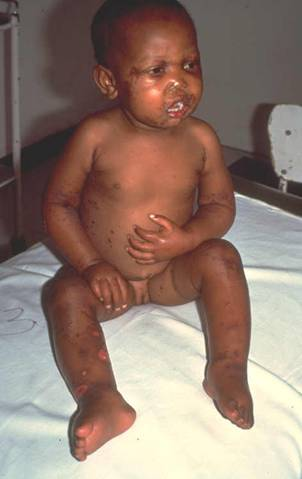
\includegraphics[width=4.19in]{images/oedema01} 

}

\caption{Child with bilateral oedema, skin and hair changes}\label{fig:unnamed-chunk-1}
\end{figure}

\begin{figure}

{\centering 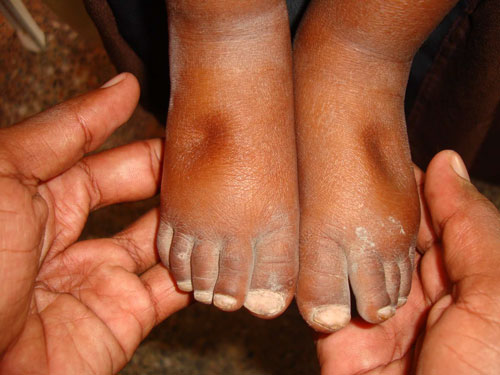
\includegraphics[width=6.94in]{images/oedema02} 

}

\caption{Bilateral pitting oedema}\label{fig:unnamed-chunk-1}
\end{figure}

B. Anthropometric indices

The physical signs and symptoms of acute undernutrition described above
are considered pathognomonic of the condition i.e., if these signs and
symptoms are found in a child, it is very likley that the child has
acute undernutrition. However, other than physical signs, there are
anthropometric indices used to diagnose acute undernutrition in
children.

\begin{enumerate}
\def\labelenumi{\arabic{enumi}.}
\tightlist
\item
  Weight-for-height/weight-for-length
\end{enumerate}

The first independent criteria for \emph{marasmus} or \emph{wasting} is
weight-for-height (WFH)/weight-for-length (WFL). Given \emph{child A},
this child's weight is assessed against the mean weight of a standard
group of children in good health with the same height or length as
\emph{child A} (length is measured when the child is \textless{} 85 cms
in height or \textless{} 24 months old). \emph{Child A} is expected to
have a weight close to the mean weight of the standard group of healthy
children if \emph{child A} is also healthy and is not undernourished.
However, if \emph{child A}'s weight deviates significantly farther from
the mean weight of the standard group of healthy children, \emph{child
A} is considered to have low weight for its height and therefore
considered \emph{marasmic} or \emph{wasted}. This deviation from the
mean, also called \emph{standard deviation (SD)} in statistics, is
calculated for each child whose weight and height have been measured and
is expressed in terms of \emph{z-scores}. Therefore, the anthropometric
index used for \emph{wasting} is weight-for-height z-scores (WHZ) and
classification of level of wasting is done based on the following WHZ
cut-offs:

~

\begin{longtable}[]{@{}ll@{}}
\toprule
\begin{minipage}[b]{0.34\columnwidth}\raggedright
\textbf{WHZ}\strut
\end{minipage} & \begin{minipage}[b]{0.47\columnwidth}\raggedright
\textbf{Classification}\strut
\end{minipage}\tabularnewline
\midrule
\endhead
\begin{minipage}[t]{0.34\columnwidth}\raggedright
WHZ \textless{} -2SD\strut
\end{minipage} & \begin{minipage}[t]{0.47\columnwidth}\raggedright
Global Acute malnurition (GAM)\strut
\end{minipage}\tabularnewline
\begin{minipage}[t]{0.34\columnwidth}\raggedright
-3SD \(\geq\) WHZ \textless{} -2SD\strut
\end{minipage} & \begin{minipage}[t]{0.47\columnwidth}\raggedright
Moderate acute malnutrition (MAM)\strut
\end{minipage}\tabularnewline
\begin{minipage}[t]{0.34\columnwidth}\raggedright
WHZ \textless{} -3SD\strut
\end{minipage} & \begin{minipage}[t]{0.47\columnwidth}\raggedright
Severe acute malnutrition (SAM)\strut
\end{minipage}\tabularnewline
\bottomrule
\end{longtable}

~

\begin{enumerate}
\def\labelenumi{\arabic{enumi}.}
\setcounter{enumi}{1}
\tightlist
\item
  Mid-upper arm circumference
\end{enumerate}

The other independent criteria for \emph{marasmus} or \emph{wasting} is
the \emph{mid-upper arm circumference} or \emph{MUAC}. \emph{MUAC} is a
measure of muscle mass and therefore detects loss of muscle mass due to
wasting. \emph{MUAC} is a good predictor of mortality and in many
studies, \emph{MUAC} predicted death in children better than any other
anthropometric indicator. Unlike weight-for-height, \emph{MUAC} is used
as an anthropometric index without need for standardisation. The
\emph{MUAC} cut-offs used to classify a child as being \emph{marasmic}
or \emph{wasted} are:

~

\begin{longtable}[]{@{}ll@{}}
\toprule
\begin{minipage}[b]{0.34\columnwidth}\raggedright
\textbf{MUAC (mm)}\strut
\end{minipage} & \begin{minipage}[b]{0.47\columnwidth}\raggedright
\textbf{Classification}\strut
\end{minipage}\tabularnewline
\midrule
\endhead
\begin{minipage}[t]{0.34\columnwidth}\raggedright
MUAC \textless{} 125\strut
\end{minipage} & \begin{minipage}[t]{0.47\columnwidth}\raggedright
Global Acute malnurition (GAM)\strut
\end{minipage}\tabularnewline
\begin{minipage}[t]{0.34\columnwidth}\raggedright
115 \(\geq\) MUAC \textless{} 125\strut
\end{minipage} & \begin{minipage}[t]{0.47\columnwidth}\raggedright
Moderate acute malnutrition (MAM)\strut
\end{minipage}\tabularnewline
\begin{minipage}[t]{0.34\columnwidth}\raggedright
MUAC \textless{} 115\strut
\end{minipage} & \begin{minipage}[t]{0.47\columnwidth}\raggedright
Severe acute malnutrition (SAM)\strut
\end{minipage}\tabularnewline
\bottomrule
\end{longtable}

~

\begin{enumerate}
\def\labelenumi{\arabic{enumi}.}
\setcounter{enumi}{2}
\tightlist
\item
  Oedema test
\end{enumerate}

The final index for acute undernutrition is \emph{oedema testing} for
\emph{kwarshiorkor} cases. This test checks whether \emph{oedema} is
present and whether it is \emph{bilateral} and \emph{pitting}. Any sign
of bilateral pitting oedema, regardless of WHZ or MUAC classification,
is considered \emph{severe acute malnutrition}.

\hypertarget{chronic-undernutrition}{%
\subsection{Chronic undernutrition}\label{chronic-undernutrition}}

Childhood \textbf{chronic undernutrition} is a condition related to a
child's exposure to inadequate nutrition over a long period of time
leading to failure of linear growth. Stunted growth reflects a process
of failure to reach linear growth potential as a result of suboptimal
health and/or nutritional conditions.

~

A. Physical signs and symptoms

A child suffering from chronic undernutrition is also called
\emph{stunting/stunted}. Such a child is said to be short for its age
(see below).

~

B. Anthropometric indices

Like with acute undernutrition, an index is used to classify whether a
child has chronic malnutrition or not. This index is called
height-for-age (HFA) or length-for-age (LFA). Given \emph{child B}, this
child's length/height is assessed against the mean length/height of a
standard group of children in good health with the same age as
\emph{child B}. \emph{Child B} is expected to have a length/height close
to the mean length/height of the standard group of healthy children if
\emph{child B} is also health and well-nourished. However, if
\emph{child B}'s length/height deviates significantly farther from the
mean height of the standard group of healthy children, \emph{child B} is
considered to have low height for its age and therefore considered to be
\emph{stunting} or \emph{stunted}. This deviation from the mean, also
called \emph{standard deviation (SD)} in statistics, is calculated for
each child whose height has been measured and is expressed in terms of
\emph{z-scores}. Therefore, the anthropometric index used for
\emph{stunting/stuntedness} is height-for-age z-scores (HAZ) and
classification of level of stunting/stuntedness is done based on the
following WHZ cut-offs:

~

\begin{longtable}[]{@{}ll@{}}
\toprule
\begin{minipage}[b]{0.34\columnwidth}\raggedright
\textbf{HAZ}\strut
\end{minipage} & \begin{minipage}[b]{0.47\columnwidth}\raggedright
\textbf{Classification}\strut
\end{minipage}\tabularnewline
\midrule
\endhead
\begin{minipage}[t]{0.34\columnwidth}\raggedright
HAZ \textless{} -2SD\strut
\end{minipage} & \begin{minipage}[t]{0.47\columnwidth}\raggedright
Global stunting/stuntedness\strut
\end{minipage}\tabularnewline
\begin{minipage}[t]{0.34\columnwidth}\raggedright
-3SD \(\geq\) HAZ \textless{} -2SD\strut
\end{minipage} & \begin{minipage}[t]{0.47\columnwidth}\raggedright
Moderate stunting/stuntedness\strut
\end{minipage}\tabularnewline
\begin{minipage}[t]{0.34\columnwidth}\raggedright
HAZ \textless{} -3SD\strut
\end{minipage} & \begin{minipage}[t]{0.47\columnwidth}\raggedright
Severe stunting/stuntedness\strut
\end{minipage}\tabularnewline
\bottomrule
\end{longtable}

~

\hypertarget{performing-anthropometric-measurements}{%
\section{Performing anthropometric
measurements}\label{performing-anthropometric-measurements}}

As described in this chapter, to be able to assess the anthropometric
indices for acute and chronic undernutrition four (4) anthropometric
measurements needs to be collected: 1) \emph{weight}; 2) \emph{height};
3) \emph{mid-upper arm circumference (MUAC)}; and, 4) \emph{oedema}. In
addition to these anthropometric measurements, information on the
child's \emph{age (in months)} and \emph{sex} will also be needed to be
able to determine the appropriate reference standards to use in
calculating the child's corresponding anthropometric indices. The next
chapters provide detailed directions on how to perform the various
anthropometric measurements accurately.

\hypertarget{weight}{%
\chapter{Measuring weight}\label{weight}}

\hypertarget{equipment}{%
\section{Equipment}\label{equipment}}

Weighing scales are the equipment needed for measuring weight.

\hypertarget{types-of-weighing-scales}{%
\subsection{Types of weighing scales}\label{types-of-weighing-scales}}

Various types of scales are available to measure the weight of a child:
1) \emph{spring scales}; 2) \emph{hanging scales}; 2) \emph{beam balance
scales}; and, 3) \emph{digital scales}.

\emph{Spring scales} are the most common type of scales used worldwide.
\emph{Hanging scales} are a kind of \emph{spring scale} that is hung
from a height instead of laid flat on the ground. \emph{Hanging scales}
are commonly preferred in many countries because they can be transported
easily, can be used in almost any setting (particularly where a flat
surface is not available) and are relatively inexpensive. However, they
are not very accurate and as such are not recommended for use in
nutrition surveys.

\begin{figure}

{\centering 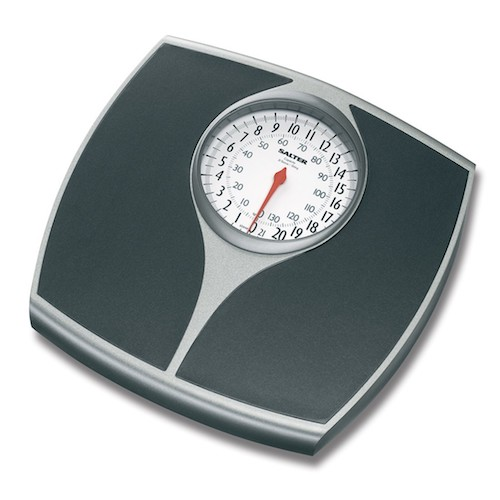
\includegraphics[width=6.94in]{images/springScale} 

}

\caption{Bathroom scale (spring)}\label{fig:weight1}
\end{figure}

\begin{figure}

{\centering 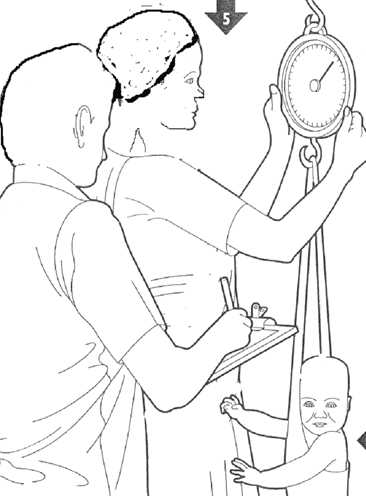
\includegraphics[width=5.08in]{images/hangingScale} 

}

\caption{Hanging scale (spring)}\label{fig:weight2}
\end{figure}

\emph{Balance beam scales} are commonly used in health centers, as they
need to be positioned on a flat surface for accurate measurement and are
not easily transported.

\begin{figure}

{\centering 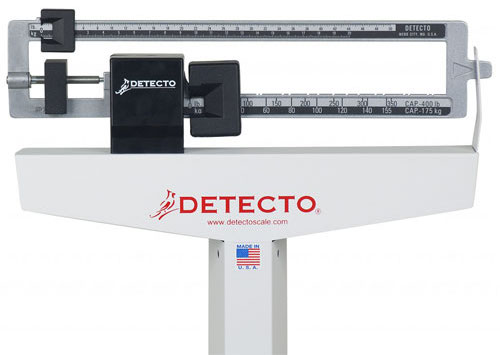
\includegraphics[width=6.94in]{images/balanceBeam} 

}

\caption{Balance beam scales}\label{fig:weight3}
\end{figure}

\emph{Digital scales} on the other hand are highly accurate (for as long
as it is powered adequately and consistently), easily transportable
though requiring a flat surface on which to be laid upon. They are
generally of high quality and rugged for frequent field use as is needed
for a nutrition survey. This is why \emph{digital scales} are what's
currently recommended for use in anthropometric measurements in a field
survey setting.

In addition to being a \emph{digital scale}, it is recommended to weigh
children using a scale with the following features:

\begin{itemize}
\item
  Solidly built and durable
\item
  Electronic (digital reading)
\item
  Measures up to 150 kg
\item
  Measures to a precision of 0.1 kg (100g)
\item
  Allows tared weighing
\end{itemize}

\textbf{``Tared weighing''} means that the scale can be re-set to zero
(\emph{``tared''}) with the person just weighed still on it. Thus, a
mother can stand on the scale, be weighed, and the scale tared. While
remaining on the scale, if she is given her child to hold, the child's
weight alone appears on the scale.

\emph{Digital scales} that allow for \textbf{tared weighing} have very
clear advantages:

\begin{itemize}
\item
  There is no need to subtract weights to determine the child's weight
  alone (reducing the risk of error).
\item
  The child is likely to remain calm when held in the mother's arms for
  weighing.
\end{itemize}

Currently, the most commonly used digital tared weighing scale is the
\textbf{UNICEF Electric Scale (UNISCALE)} which is produced by
\textbf{SECA} (the non-UNICEF branded scale is the \textbf{SECA model
890} or \textbf{SECA model 874})

\begin{figure}

{\centering 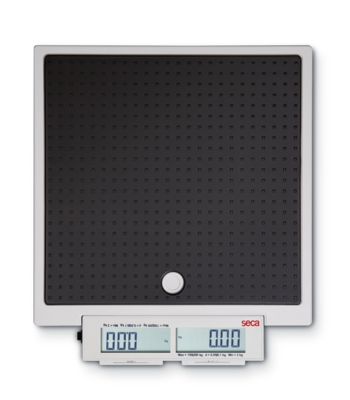
\includegraphics[width=4.86in]{images/seca874} 

}

\caption{SECA scale model 874}\label{fig:weight4}
\end{figure}

\hypertarget{general-use-care-and-maintenance-of-seca-tared-scales}{%
\subsection{General use, care and maintenance of SECA tared
scales}\label{general-use-care-and-maintenance-of-seca-tared-scales}}

\begin{enumerate}
\def\labelenumi{\arabic{enumi}.}
\tightlist
\item
  Place the scale on a hard, level surface (wood, concrete, or firm
  earth). Soft or uneven surfaces may cause small errors in weighing. It
  is therefore advisable that each survey team are provided with a
  wooden plank that can be laid on top of unlevel ground as a way to
  even out the surface. The plank should be big enough to cover a
  reasonable surface and sturdy enough to carry the weight of the scale
  and those being weighed.
\end{enumerate}

\begin{figure}

{\centering 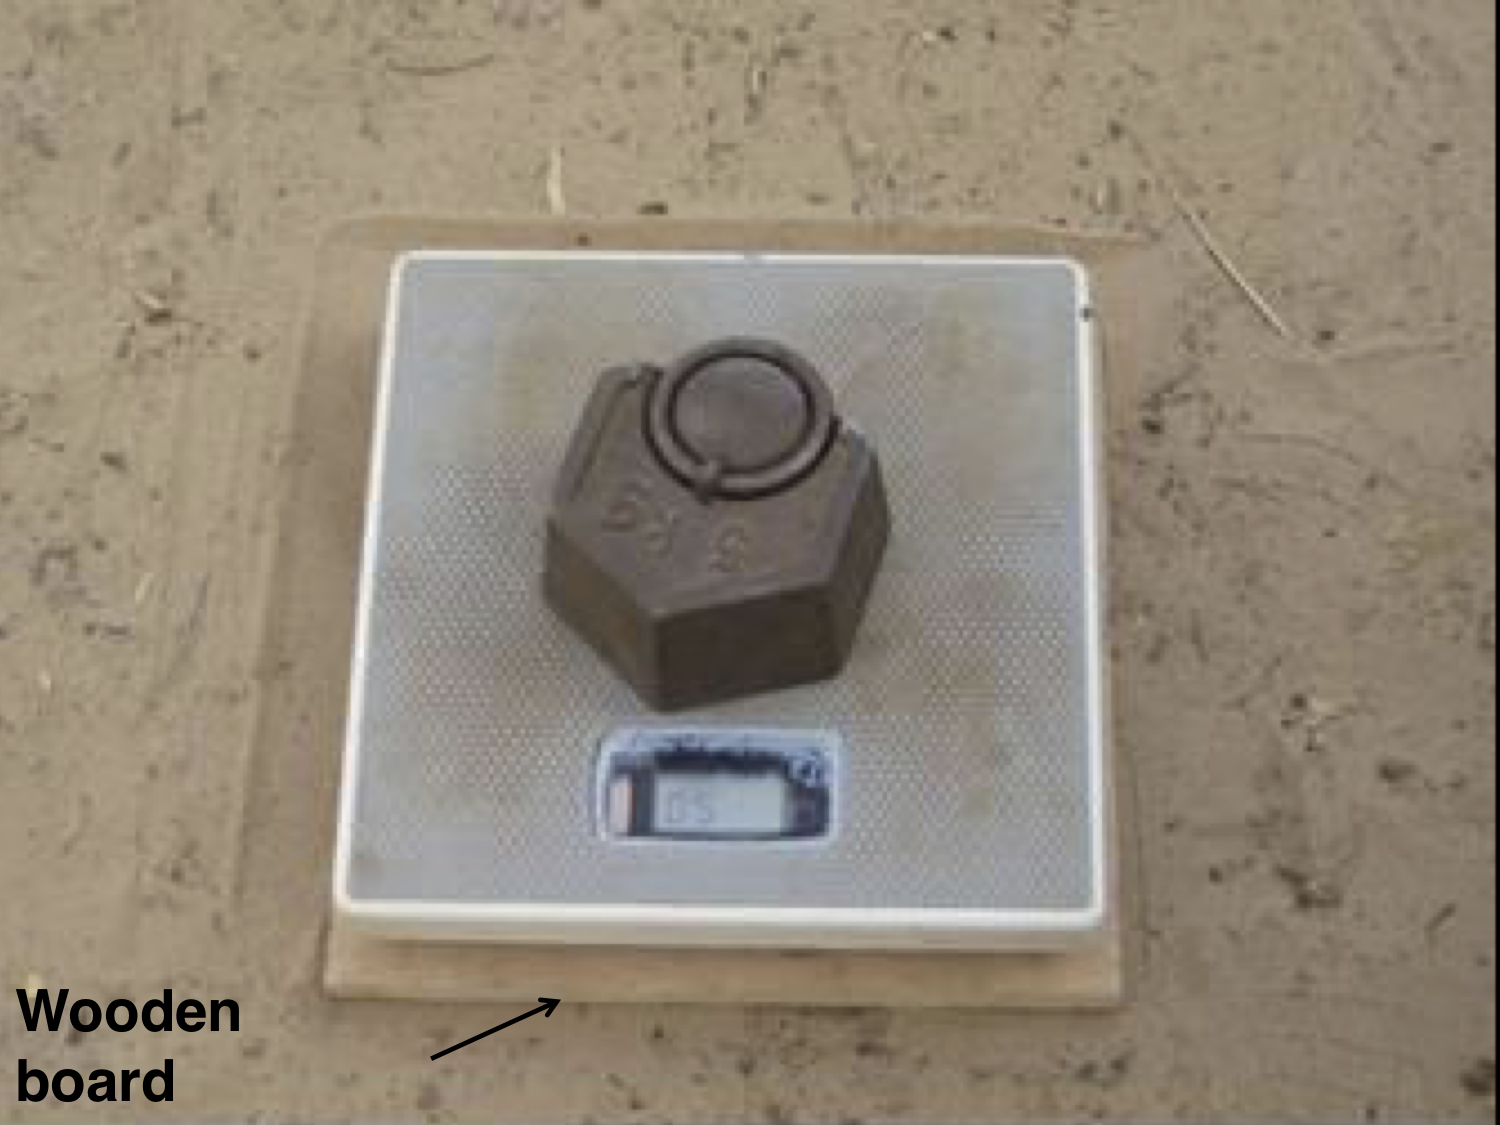
\includegraphics[width=0.5\linewidth]{images/weight01} 

}

\caption{Weighing scale on a wooden plank}\label{fig:weight5}
\end{figure}

\begin{enumerate}
\def\labelenumi{\arabic{enumi}.}
\setcounter{enumi}{1}
\item
  The scale will not function correctly if it becomes too warm. It is
  best to use the scale in the shade, or indoors. If the scale becomes
  hot and does not work correctly, place it in a cooler area and wait 15
  minutes before using again.
\item
  The scale must adjust to changes in temperature. If the scale is moved
  to a new site with a different temperature, wait for 15 minutes before
  using the scale again. It is advisable to test the scale before every
  measurement when the scale is moved and operated in extreme weather
  conditions.
\item
  The scale must be tested every single day of fieldwork. This is best
  done using a labelled standard weight of 2.5 - 5.0 kg. This can be
  purchased locally, but must be tested initially to ensure that the
  indicated weight is accurate. Record the results of the daily test of
  the scale, including the date and weight. Using other types of
  standard weights is possible, but is not recommended. Some surveys
  have in the past used filled water bottles for testing, but as water
  or other liquids evaporate, this technique is flawed. Sand is a viable
  alternative, but only if labelled weights are not available.
\item
  Handle the scale carefully:

  \begin{itemize}
  \tightlist
  \item
    Do not drop or bump the scale.
  \item
    Do not weigh loads with a total weight of more than 150 kg.
  \item
    Do not store the scale in direct sunlight or other hot places.
  \item
    Protect the scale against excess humidity or wetness.
  \item
    Do not use the scale at temperatures below 10º C or above 45º C.
  \end{itemize}
\item
  The scale is battery-powered. Around 120,000 weighings can be
  performed with a fresh set of batteries.
\end{enumerate}

\hypertarget{personnel}{%
\section{Personnel}\label{personnel}}

At least two trained personnel are required when performing weight
measurement. One is assigned as the \textbf{measurer} while the other is
assigned as the \textbf{assistant}. It is important that prior to the
measurement of the weight of a child that these roles are clearly
specified and that each personnel knows what their role entails.
Switching roles between measurement of different children is acceptable
for as long as all personnel are trained on performing the tasks
expected of either \textbf{measurer} or \textbf{assistant}. For specific
tasks for each role, see next section.

\hypertarget{steps-in-weighing-a-child}{%
\section{Steps in weighing a child}\label{steps-in-weighing-a-child}}

\begin{enumerate}
\def\labelenumi{\arabic{enumi}.}
\tightlist
\item
  \emph{Prepare the child for weighing}
\end{enumerate}

Explain to parents/caretakers that the child needs to remove outer
clothing in order to obtain an accurate weight. A wet diaper, or shoes
and jeans, can contribute substantially to the measured weight (up to
0.5 kgs) making the measurement inaccurate. Babies should be weighed
naked but precautions needs to be put in place to ensure that the baby
stay warm while waiting to be weighed and while they are being weighed.
They can be wrapped in a blanket to keep them warm while waiting. When
being weighed, the adult can be weighed holding a blanket that can be
used to wrap around the naked baby during measurement. Older children
should remove all but minimal clothing, such as their underclothes.

If it is too cold to undress a child or if the child resists being
undressed and becomes agitated, please weigh the clothed child, but
indicate in the questionnaire that the child could not be undressed to
the minimum and take a note of the circumstances. To be able to adjust
the weight of clothed children, weigh one set of child's clothing
separately and record. This weight will be used in adjusting the weight
measurement of all children weighed with clothes on.

\begin{enumerate}
\def\labelenumi{\arabic{enumi}.}
\setcounter{enumi}{1}
\tightlist
\item
  \emph{Switch on scale}
\end{enumerate}

The \textbf{measurers} should switch on the scale with no weight
applied. The \textbf{SECA 874} can be turned on by tapping the
\textbf{start} button. The \textbf{SECA 890} can be turned on by
covering the solar cells for less than a second.

\begin{figure}

{\centering 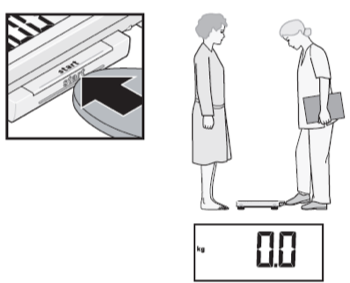
\includegraphics[width=4.86in]{images/seca874start} 

}

\caption{Turning on the SECA 874}\label{fig:weight6}
\end{figure}

\begin{figure}

{\centering 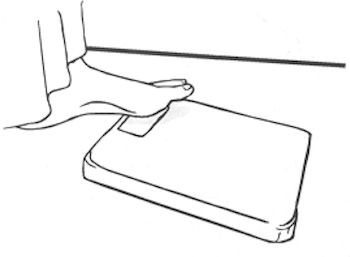
\includegraphics[width=4.86in]{images/seca890start} 

}

\caption{Turning on the SECA 890}\label{fig:weight7}
\end{figure}

When the \textbf{SECA 890} is switched on, you will first notice the
display showing \texttt{188.8}. Wait for the display to turn
\texttt{0.0} before putting any weight onto the scale. The
\textbf{assistant} on the other hand will be holding onto the paper
questionniare or the mobile device. The \textbf{assistant} will be in
charge of recording the weight measurement.

\begin{figure}

{\centering 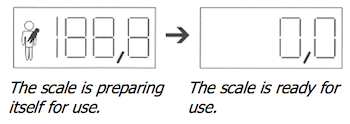
\includegraphics[width=4.86in]{images/seca890zero} 

}

\caption{SECA 890 ready}\label{fig:weight8}
\end{figure}

\begin{enumerate}
\def\labelenumi{\arabic{enumi}.}
\setcounter{enumi}{2}
\tightlist
\item
  \emph{Weighing the child}
\end{enumerate}

This step differs between children who are able to stand still on the
scale long enough for a measurement to be read and recorded and children
who are too young to do so. Generally, children 2 years and above should
be able to stand on the scale still on their own long enough. However,
it is to the discretion of the \textbf{measurer} whether this is the
case or not.

\begin{enumerate}
\def\labelenumi{\alph{enumi}.}
\tightlist
\item
  \emph{Weigh child on scale on their own}
\end{enumerate}

If child is able to stand still on the scale long enough, the child can
be weighed alone. \textbf{Measurer} should explain to the child that
he/she will need to step on to the scale alone and standing very still.
\textbf{Measurer} will ask the child to stand in the middle of the
scale, feet slightly apart and to remain still until the weight appears
and that the measurement is retained on the display (about 3 seconds
that the measurement is stable with child standing still and not moving
the display will stop flashing signifying that the weight display has
been stored). It is important that no one holds or supports the child
until a weight measurement has been retained on the display successfully
as this will interfere with the measurement. If the child does not stand
still or is unable or does not want to stand on his/her own, then step b
below should performed instead.

The \textbf{measurer} then reads out loud the child's weight from the
display. The \textbf{measurer} should read the measurement entirely
including the one decimal place that shows in display (to the nearest
0.1 kg). Note that when using the SECA 874, the weight is displayed with
two decimal places but the second decimal number is always 0. The second
decimal place is not recorded.

The \textbf{assistant} then repeats the weight that has been called out.

The \textbf{measurer} then confirms if this is the correct weight. If
correct, then the \textbf{assistant} records the weight measurement on
the paper questionnaire or on the mobile device. If incorrect,
\textbf{measurer} reads out the measurement again until the
\textbf{assistant} is able to repeat the correct weight.

The child can then step off the scale.

\begin{enumerate}
\def\labelenumi{\alph{enumi}.}
\setcounter{enumi}{1}
\tightlist
\item
  \emph{Tared weighing}
\end{enumerate}

If child is unable to stand still on the scale long enough or if child
doesn't want to stand on the scale alone, then this child should be
measured using \emph{tared weighing}.

The \textbf{measurer} asks the mother/caretaker to step onto the scale
and then to stand still. After about 3 seconds, the weight of the
mother/caretaker will be displayed.

\begin{figure}

{\centering 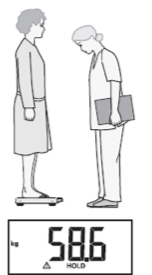
\includegraphics[width=2.11in]{images/seca874adult} 

}

\caption{Weighing the adult first on the SECA 874}\label{fig:weight9}
\end{figure}

If using the \textbf{SECA 874}, the \textbf{measurer} will have to press
the \textbf{2 in 1} key found on the scale. This will store the weight
of the mother/caretaker. The display on the device would show
\texttt{0.0} reading and the word \textbf{NET} indicating that the
weight of the mother/caretaker has been stored.

\begin{figure}

{\centering 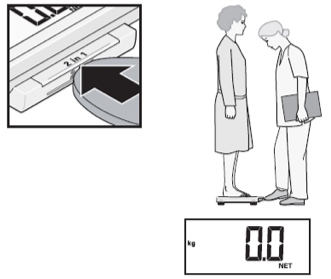
\includegraphics[width=4.6in]{images/seca874net} 

}

\caption{Taring the SECA 874}\label{fig:weight10}
\end{figure}

If using the \textbf{SECA 890}, the \textbf{measurer} will have to cover
the solar cell of the device for less than a second and the display will
revert back to \texttt{0.0} reading. This indicates that the weight of
the mother/caretaker has been stored.

\begin{figure}

{\centering 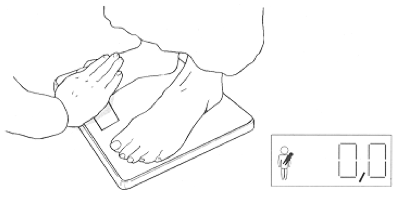
\includegraphics[width=5.51in]{images/seca890cover} 

}

\caption{Taring the SECA 890}\label{fig:weight11}
\end{figure}

The \textbf{measurer} then asks the mother/caretaker to hold/carry the
baby/child on their arms and to again stand as still as possible. The
display will show a weight measure. If the weight display and the
message \texttt{HOLD} are flashing, it means that the scale is waiting
for the measurement to stabilise. The \textbf{measurer} should wait for
the weight display and the message \texttt{HOLD} to stop flashing before
reading the weight measurement.

\begin{figure}

{\centering 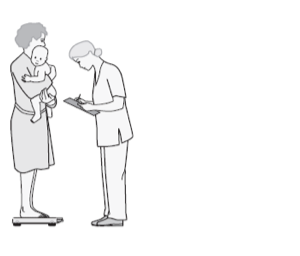
\includegraphics[width=3.32in]{images/seca874hold} 

}

\caption{SECA 874 on hold}\label{fig:weight12}
\end{figure}

Once the weight display has stopped flashing, The \textbf{measurer}
reads out loud the child's weight from the display. The
\textbf{measurer} should read the measurement entirely including the one
decimal place that shows in display. Note that when using the SECA 874,
the weight is displayed with two decimal places but the second decimal
number is always 0. The second decimal place is not recorded.

The \textbf{assistant} then repeats the weight that has been called out.

The \textbf{measurer} then confirms if this is the correct weight. If
correct, then the \textbf{assistant} records the weight measurement on
the paper questionnaire or on the mobile device. If incorrect,
\textbf{measurer} reads out the measurement again until the
\textbf{assistant} is able to repeat the correct weight.

\BeginKnitrBlock{rmdremind}
\item 

Always calibrate scales ever day in the morning before data collection.

\item 

Always measure weight before height.

\item 

If there is more than 1 eligible child in a household, always weigh the
less agitated one first.

\item 

Try and obtain scales that are sturdy but light enough to be carried
easily by the team.

\item 

Measure weight without clothes.
\EndKnitrBlock{rmdremind}

\hypertarget{height}{%
\chapter{Measuring height}\label{height}}

\hypertarget{equipment-1}{%
\section{Equipment}\label{equipment-1}}

A height board, sometimes called a heightometer or stadiometer, is the
tool used to measure height of children. It is usually constructed based
on a ruler with a sliding horizontal headpiece which adjusts to rest on
top of the head. Some common types of height boards are the wooden
2-piece and wooden 3-piece, plastic free-standing, aluminum
free-standing and locally-produced boards. Of these, it is preferable to
use wooden measuring boards as opposed to aluminum boards which can get
very hot in the sun and burn children. The measuring board should be at
least 130 cm long and made of hardwood with a hard water-resistant
finish. Choice of woods is important. The board should be light enough
to be easily carried in the field from house to house. The board should
have two tape measures attached to it, one on each side, and they should
be marked out in 0.1 cm increments. The board should be easily set
upright to measure height with the head piece of the length board
becoming the base when the board is set upright.

\begin{figure}

{\centering 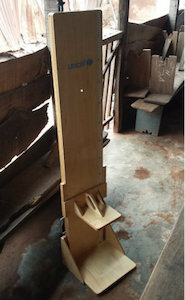
\includegraphics[width=2.57in]{images/heightBoard01} 

}

\caption{2-piece height board standing up}\label{fig:height01}
\end{figure}

\begin{figure}

{\centering 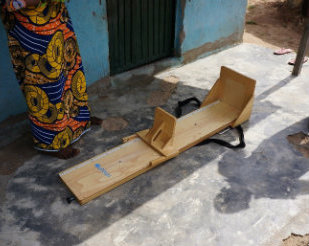
\includegraphics[width=4.29in]{images/heightBoard02} 

}

\caption{2-piece height board lying down}\label{fig:height02}
\end{figure}

\begin{figure}

{\centering \includegraphics[width=3.42in]{images/shorrBrdcarry} 

}

\caption{2-piece height board folded and carried}\label{fig:height03}
\end{figure}

\hypertarget{personnel-1}{%
\section{Personnel}\label{personnel-1}}

A minimum of two personnel are needed to measure the height or length of
a child. If human resources are not an issue, a three-person team would
be ideal especially when taking the length of the child. For a
two-person team, one is assigned as the \textbf{measurer} while the
other is assigned as the \textbf{assistant}. It is important that prior
to the measurement of the height of a child that these roles are clearly
specified and that each personnel knows what their role entails.
Switching roles between measurement of different children is acceptable
for as long as all personnel are trained on performing the tasks
expected of either \textbf{measurer} or \textbf{assistant}. For specific
tasks for each role, see next section.

\hypertarget{steps-in-measuring-length-or-height-of-child}{%
\section{Steps in measuring length or height of
child}\label{steps-in-measuring-length-or-height-of-child}}

Depending on the age of the child, either the weight or the length is
measured. For children less than 24 months old (or for height less than
85 cms), length should be measured i.e., height board on recumbent
position with the child lying down using a length board which should be
placed on a flat, stable surface such as a table.

\begin{figure}

{\centering 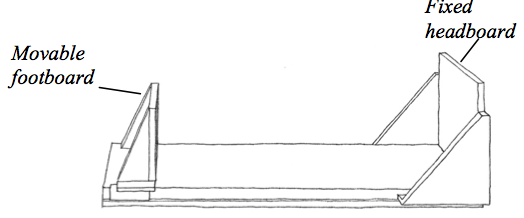
\includegraphics[width=7.28in]{images/heightBoard03} 

}

\caption{Length board flat on a stable surface}\label{fig:height04}
\end{figure}

For children 24 months and older, height should be measured i.e., height
board on the vertical position with the child standing up (unless child
is unable to stand). Use a height board mounted at a right angle between
a level floor and against a straight, vertical surface such as a wall or
pillar.

\begin{figure}

{\centering 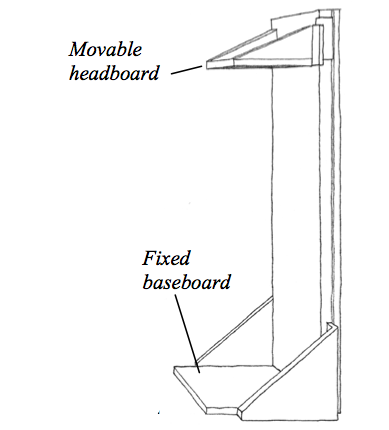
\includegraphics[width=5.4in]{images/heightBoard04} 

}

\caption{Height board mounted upright}\label{fig:height05}
\end{figure}

Measuring children standing up is much easier. Length is much more
difficult to measure than height.

Standing height is about 0.7 cm less than recumbent length. This
difference was taken into account in developing the WHO growth
standards. Therefore, it is important to adjust the measurements if
length is taken instead of height, and vice versa.

\begin{itemize}
\item
  If a child less than 2 years old will not lie down for measurement of
  length, measure standing height and add 0.7 cm to convert it to
  length.
\item
  If a child aged 2 years or older cannot stand, measure recumbent
  length and subtract 0.7 cm to convert it to height.
\end{itemize}

It is recommended that this adjustment to not be made by enumerators
during the survey. Instead, an entry in the data collection form /
survey instrument should be included that indicates whether measurement
made was a height or a length measurement. This will allow adjustments
to be made to the height/length measurements post-survey.

\hypertarget{measuring-height}{%
\subsection{Measuring height}\label{measuring-height}}

\begin{figure}

{\centering 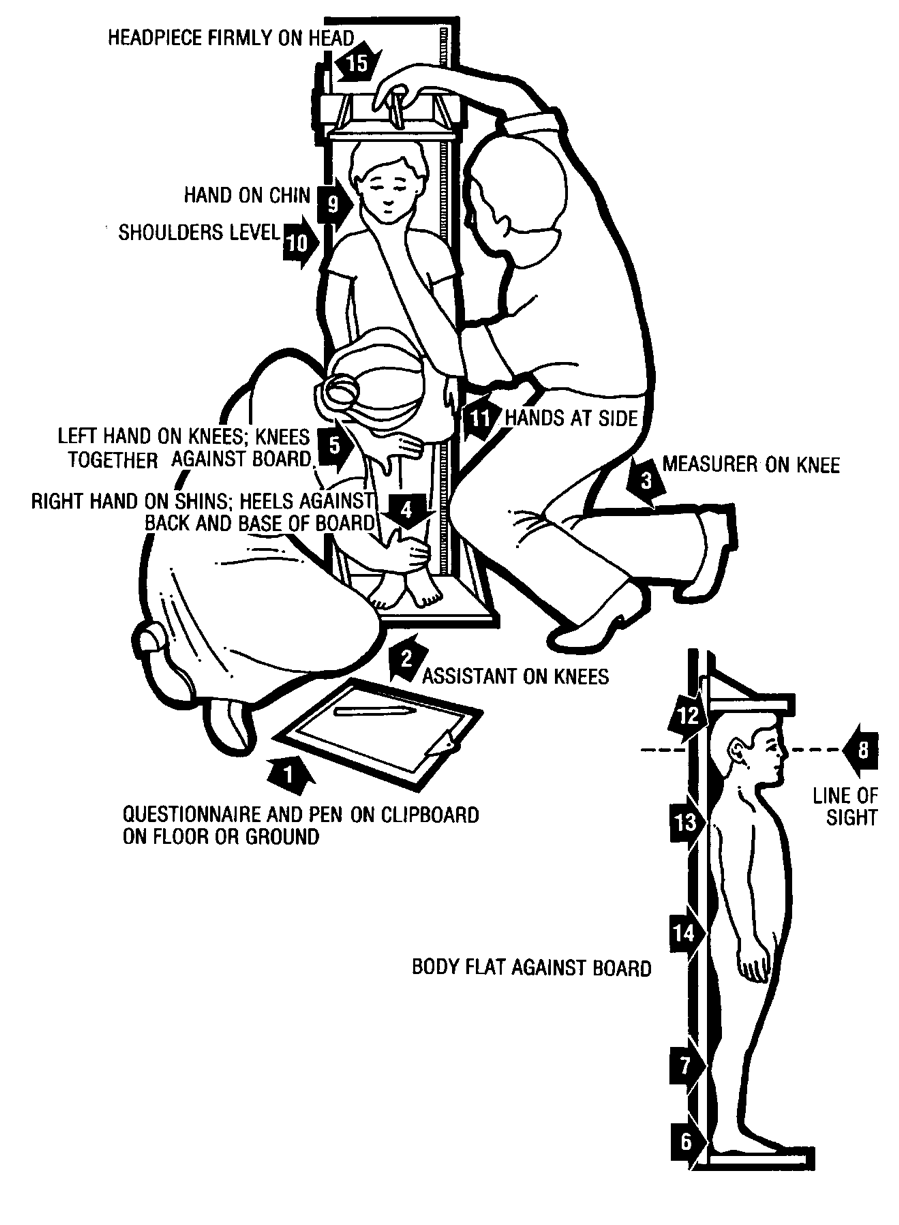
\includegraphics[width=12.49in]{images/height} 

}

\caption{Steps in measuring height}\label{fig:height06}
\end{figure}

\begin{enumerate}
\def\labelenumi{\arabic{enumi}.}
\item
  \textbf{Measurer} or \textbf{Assistant} should place the measuring
  board on a hard flat surface against a wall, table, tree, staircase,
  etc. Make sure the board is stable. Check that shoes, socks and hair
  ornaments have been removed.
\item
  \textbf{Measurer} or \textbf{Assistant} should ask the mother to
  remove the child's shoes and unbraid any hair that would interfere
  with the height measurement. Ask mother to walk the child to the board
  and to kneel in front of the child.
\item
  \textbf{Assistant} should place the paper questionnaire or mobile
  device on the ground (\textbf{arrow 1}) and kneel with both knees on
  the right side of the child (\textbf{arrow 2}).
\item
  \textbf{Measurer} should kneel on their right knee only, for maximum
  mobility, on the child's left side (\textbf{arrow 3}).
\item
  \textbf{Assistant} should place the child's feet flat and together in
  the centre of and against the back and base of the board. The
  assistant should place right hand just above the child's ankles on the
  shins (\textbf{arrow 4}) with left hand on the child's knees
  (\textbf{arrow 5}) and push against the board making sure the child's
  legs are straight and the heels and calves are against the board
  (\textbf{arrows 6} and \textbf{7}). The \textbf{assistant} then
  notifies the measurer when positioning of the feet and legs is
  complete.
\item
  \textbf{Measurer} tells the child to look straight ahead at the mother
  if she is in front of the child. Make sure the child's line of sight
  is level with the ground (\textbf{arrow 8}). \textbf{Measurer} places
  open left hand on the child's chin and gradually closes hand
  (\textbf{arrow 9}) taking care that the child's mouth or ears are not
  covered. The \textbf{measurer} makes sure the shoulders are level
  (\textbf{arrow 10}), the hands are at the child's side
  (\texttt{arrow\ 11}), and the head, shoulder blades and buttocks are
  against the board (\textbf{arrows 12}, \textbf{13} and \textbf{14}).
  With the right hand, the \textbf{measurer} lowers the headpiece on top
  of the child's head making sure that the headpiece pushes through the
  child's hair (\textbf{arrow 15}).
\item
  \textbf{Measurer} and \textbf{Assistant} should check the child's
  position (\textbf{arrow 1-15}) and repeating any steps necessary.
\item
  When the child's position is correct, the \textbf{measurer} reads and
  calls out the measurement to the nearest 0.1cm. Then, the
  \textbf{measurer} removes the headpiece from the child's head and
  releases the left hand from the child's chin and supports the child
  during the recording.
\item
  \textbf{Assistant} immediately records the measurement and shows it to
  the \textbf{measurer}.
\item
  \textbf{Measurer} checks the recorded measurement on the questionnaire
  for accuracy and legibility and instructs the \textbf{assistant} to
  erase and correct any errors.
\end{enumerate}

\BeginKnitrBlock{rmdnote}
If you are unsure or not confident in the precision of the child's age
(over age 2), please take measurement as described above. If the child's
height is measured to less than 85 cm, you must instead measure the
child's length (see \protect\hyperlink{measuring-length}{Measuring
length}).
\EndKnitrBlock{rmdnote}

\BeginKnitrBlock{rmdwarning}
Common mistakes when measuring height include 1) child leaning to one
side; 2) heels not touching the board; 3) hands not at side.
\EndKnitrBlock{rmdwarning}

\hypertarget{measuring-length}{%
\subsection{Measuring length}\label{measuring-length}}

\begin{figure}

{\centering 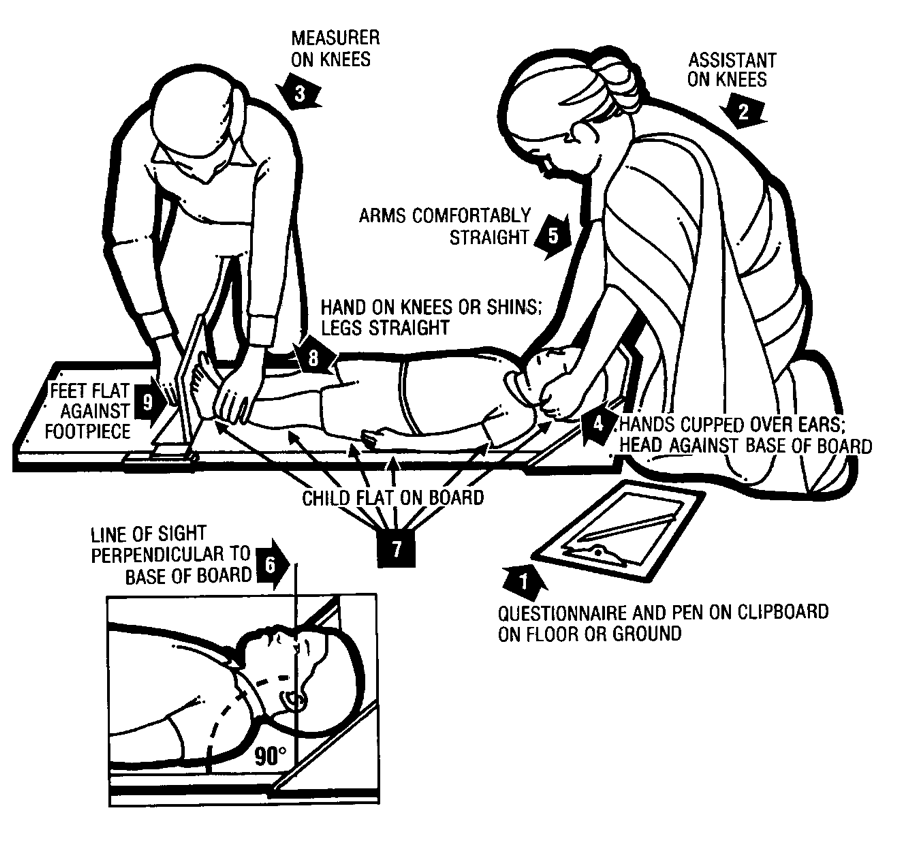
\includegraphics[width=12.46in]{images/length} 

}

\caption{Steps in measuring length}\label{fig:height07}
\end{figure}

\begin{enumerate}
\def\labelenumi{\arabic{enumi}.}
\item
  \textbf{Measurer} or \textbf{assistant} places the measuring board on
  a hard flat surface, such as the ground, floor or a steady table.
  Cover the length board with a thin cloth or soft paper for hygiene and
  for the baby's comfort.
\item
  \textbf{Assistant} places the paper questionnaire or the mobile device
  on the ground, floor or table (\textbf{arrow 1}) and kneels with both
  knees behind the base of the board, if it is on the ground or floor
  (\textbf{arrow 2}).
\item
  \textbf{Measurer} kneels on the child's right side and holds the
  footpiece with right hand (\textbf{arrow 3}).
\item
  With the mother's/caretaker's help, the \textbf{measurer} and
  \textbf{assistant} should lay the child on the board. The
  \textbf{assistant} should support the back of the child's head with
  hands and gradually lower the child onto the board. The
  \textbf{measurer} on the other hand supports the child at the trunk of
  the body.
\item
  \textbf{Measurer} or \textbf{assistant} asks the mother/caretaker to
  kneel on the opposite side of the board facing the measurer to help
  keep the child calm.
\item
  \textbf{Assistant} cups hands over the child's ears (\textbf{arrow
  4}). With arms comfortably straight (\textbf{arrow 5}),
  \textbf{assistant} places the child's head against the base of the
  board so that the child is looking straight up. The child's line of
  sight should be perpendicular to the ground (\textbf{arrow 6}). The
  \textbf{assistant's} head should be straight over the child's head and
  looking directly into the child's eyes.
\end{enumerate}

\begin{figure}

{\centering 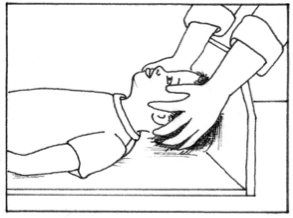
\includegraphics[width=4.07in]{images/heightBoard05} 

}

\caption{Positioning child's head against the base of the board}\label{fig:height08}
\end{figure}

\begin{enumerate}
\def\labelenumi{\arabic{enumi}.}
\setcounter{enumi}{6}
\tightlist
\item
  \textbf{Measurer} makes sure the child is lying flat and in the centre
  of the board (\textbf{arrow 7}) and places left hand on the child's
  shins (above the ankles) or on the knees (\textbf{arrow 8}) pressing
  them firmly against the board. Note that With the right hand,
  \textbf{measurer} places the footpiece firmly against the child's
  heels (\textbf{arrow 9}).
\end{enumerate}

\begin{figure}

{\centering 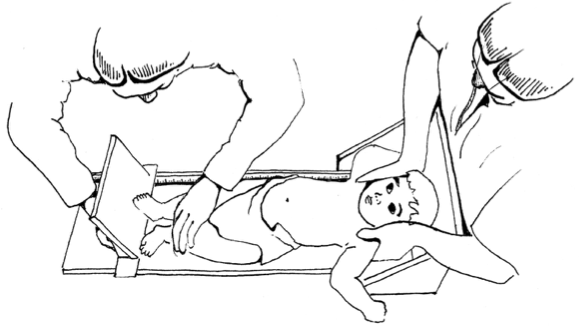
\includegraphics[width=8.04in]{images/heightBoard06} 

}

\caption{Measurer and assistant working together to position child}\label{fig:height09}
\end{figure}

\begin{enumerate}
\def\labelenumi{\arabic{enumi}.}
\setcounter{enumi}{7}
\item
  \textbf{Measurer} and \textbf{assistant} checks the child's position
  (\textbf{arrows 4-9}) and repeats any steps as necessary to correct
  child's position.
\item
  When the child's position is correct, \textbf{measurer} reads and
  calls out the measurement to the nearest 0.1 centimetre. The
  \textbf{measurer} then removes the footpiece, releases left hand from
  the child's shins or knees and supports the child during the
  recording.
\item
  The \textbf{assistant} then immediately releases the child's head,
  records the measurement on the paper questionnaire or mobile device
  and shows it to the \textbf{measurer}. Alternatively, the
  \textbf{assistant} calls out the measurement and have the
  \textbf{measurer} confirm by repeating back.
\item
  \textbf{Assistant} records whether the child was measured lying down
  or standing up.
\item
  \textbf{Measurer} checks the recorded measurement on the questionnaire
  for accuracy and legibility then instructs the assistant to cancel and
  correct any errors.
\end{enumerate}

\BeginKnitrBlock{rmdnote}
If you are unsure or not confident in the precision of the child's age
(under age 2), take measurement as described above. If the child's
length is measured to 85 cm or more, you must instead measure the
child's height (see \protect\hyperlink{measuring-height}{Measuring
height}).
\EndKnitrBlock{rmdnote}

\BeginKnitrBlock{rmdwarning}
Common mistakes when measuring length include 1) toes pointed; 2) knees
bent; 3) head lifted off the board.
\EndKnitrBlock{rmdwarning}

\BeginKnitrBlock{rmdremind}
\item 

The measuring boards should be at least 130 cm in length and be made of
treated wood.

\item 

There should be measuring tape on both sides of the measuring board.

\item 

The measuring board must be cleaned before being stored.

\item 

Record measurements to the nearest 0.1 cm.
\EndKnitrBlock{rmdremind}

\hypertarget{muac}{%
\chapter{Measuring mid-upper arm circumference (MUAC)}\label{muac}}

\hypertarget{equipment-2}{%
\section{Equipment}\label{equipment-2}}

\begin{figure}

{\centering 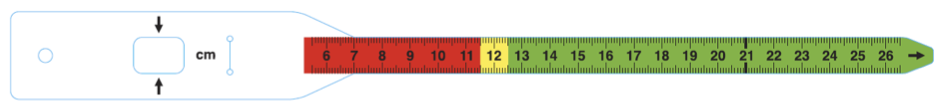
\includegraphics[width=13.11in]{images/muac01} 

}

\caption{MUAC tape with colour cut-offs at 115 mm and 125 mm}\label{fig:muac1}
\end{figure}

MUAC is a quick and simple way to determine whether or not a child is
malnourished using a simple colored plastic strip. There are different
types of MUAC tape available. All are graduated in millimetres and some
are colour coded (red, yellow and green) to indicate the nutritional
status of a child or adult. The colour codes and gradations vary
depending on the tape type.

The most appropriate MUAC tape to use would be the tapes that use the
latest WHO Growth Standards cut-offs for acute malnutrition. These are
the tapes that have three colours (red, yellow, green) with colour
cutoffs at 115 mm and 125 mm. The MUAC tapes should also be precise up
to 1 mm. The material for the MUAC tape needs to be flexible but
non-stretchable. An example of this kind of MUAC tape is shown in Figure
\ref{fig:muac1}.

\hypertarget{personnel-2}{%
\section{Personnel}\label{personnel-2}}

Only a single \textbf{measurer} is required to measure the MUAC of a
child. If with an \textbf{assistant} is available, he/she records the
MUAC measurement.

\hypertarget{steps-in-measuring-muac}{%
\section{Steps in measuring MUAC}\label{steps-in-measuring-muac}}

\begin{figure}

{\centering 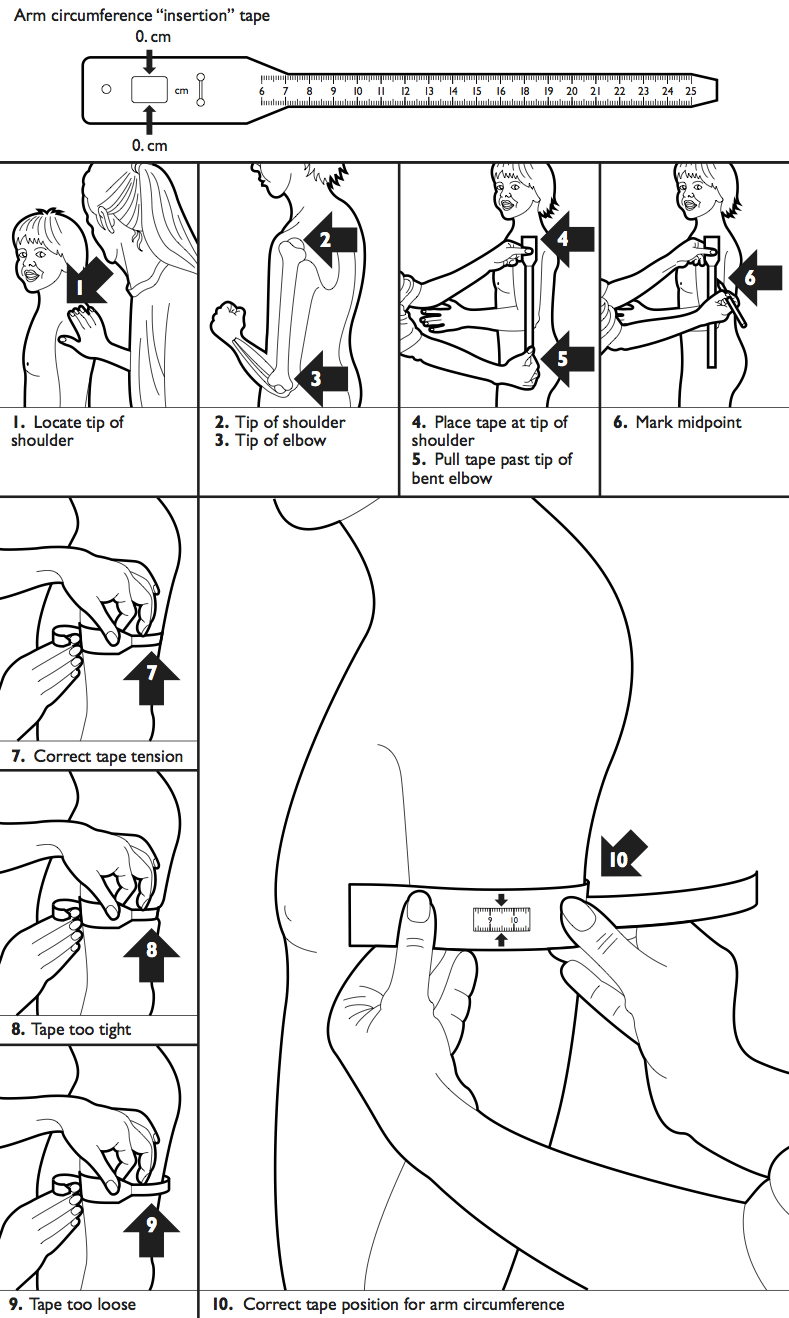
\includegraphics[width=10.96in]{images/muac02} 

}

\caption{Steps in measuring MUAC}\label{fig:muac2}
\end{figure}

\begin{enumerate}
\def\labelenumi{\arabic{enumi}.}
\item
  When measuring MUAC, ensure work at eye level. Sit down when possible.
  Very young children can be held by their mother during this procedure.
  Ask the mother to remove clothing that may cover the child's left arm.
\item
  \textbf{Measurer} calculates the midpoint of the child's left upper
  arm by first locating the tip of the child's shoulder (\textbf{arrows
  1} and \textbf{2}) with finger tips. Bend the child's elbow to make a
  right angle (\textbf{arrow 3}). Place the tape at zero, which is
  indicated by two arrows, on the tip of the shoulder (\textbf{arrow 4})
  and pull the tape straight down past the tip of the elbow
  (\textbf{arrow 5}). Read the number at the tip of the elbow to the
  nearest centimeter. Divide this number by two to estimate the
  midpoint. As an alternative, bend the tape up to the middle length to
  estimate the midpoint. A piece of string can also be used for this
  purpose. Either you or an assistant can mark the midpoint with a pen
  on the arm (\textbf{arrow 6}).
\item
  \textbf{Measurer} straightens the child's arm and wraps the tape
  around the arm at midpoint. Make sure the numbers are right side up.
  Make sure the tape is flat around the skin (\textbf{arrow 7}).
\item
  \textbf{Measurer} and \textbf{assistant} inspects the tension of the
  tape on the child's arm. Make sure the tape has the proper tension
  (\textbf{arrow 7}) and is not too tight or too loose (\textbf{arrows
  8-9}). Repeat any steps as necessary.
\item
  \textbf{Assistant} is on ready with the paper questionnaire or the
  mobile device.
\item
  When the tape is in the correct position on the arm with the correct
  tension, \textbf{measurer} reads and calls out the measurement to the
  nearest 0.1 cm. (\textbf{arrow 10}).
\item
  \textbf{Assistant} immediately records the measurement on the
  questionnaire or the mobile device and shows it to the
  \textbf{measurer}.
\item
  While the assistant records the measurement, \textbf{measurer} loosens
  the tape on the child's arm.
\item
  \textbf{Measurer} checks the recorded measurement on the questionnaire
  or mobile device for accuracy and legibility then instructs the
  assistant to erase and correct any errors.
\item
  \textbf{Measurer} removes the tape from the child's arm.
\end{enumerate}

\BeginKnitrBlock{rmdwarning}
Common mistakes when measuring MUAC include 1) measuring on the right
arm; 2) estimating (rather than measuring) the mid-point of the upper
arm; 3) bending the MUAC tape when measuring the midpoint; 4) not
measuring the midpoint from the tip of the shoulder to the elbow bend;
5) pulling the MUAC tape too tight; 6) not pulling the MUAC tape tight
enough (too slack); 7) not reading the tape accurately (to nearest
millimetre).
\EndKnitrBlock{rmdwarning}

\hypertarget{oedema}{%
\chapter{Checking for oedema}\label{oedema}}

Nutritional oedema, manifested as bilateral pitting oedema, is a sign of
severe acute malnutrition. Nutritional oedema always starts from the
feet and extends upwards to other parts of the body. Children with
nutritional oedema are at high risk of mortality hence require immediate
therapeutic care. This \protect\hyperlink{oedema}{chapter} describes how
to check nutritional oedema.

\hypertarget{equipment-3}{%
\section{Equipment}\label{equipment-3}}

No tool or equipment is needed for checking for nutritional oedema.

\hypertarget{personnel-3}{%
\section{Personnel}\label{personnel-3}}

Oedema check can be performed by a single person.

\hypertarget{steps-in-checking-for-nutritional-oedema}{%
\section{Steps in checking for nutritional
oedema}\label{steps-in-checking-for-nutritional-oedema}}

\begin{enumerate}
\def\labelenumi{\arabic{enumi}.}
\tightlist
\item
  Press both feet with thumbs
\end{enumerate}

Using both thumbs of your hands, apply normal pressure on top of both
feet of the child for about three seconds as shown below. You can
estimate three seconds by counting \textbf{\emph{`one thousand and one,
one thousand and two, one thousand and three'}} in English. It takes
roughly 3 seconds to be able to say these words.

\begin{figure}

{\centering 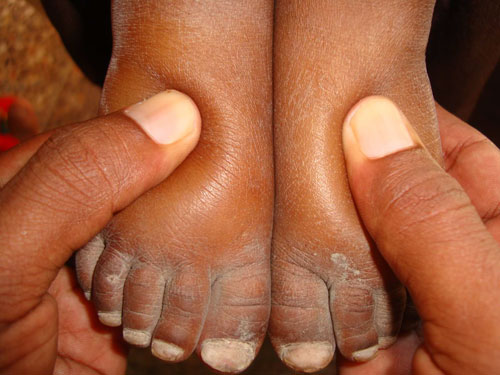
\includegraphics[width=6.94in]{images/oedemaStep1} 

}

\caption{Press both feet with thumbs}\label{fig:oedemaStep1}
\end{figure}

\begin{enumerate}
\def\labelenumi{\arabic{enumi}.}
\setcounter{enumi}{1}
\tightlist
\item
  Release pressure from feet
\end{enumerate}

After three seconds, release the pressure you are applying on the
child's feet. Observe the resulting effect on the child's feet.

If there is oedema, an impression remains on both feet for a few seconds
as shown below.

\begin{figure}

{\centering 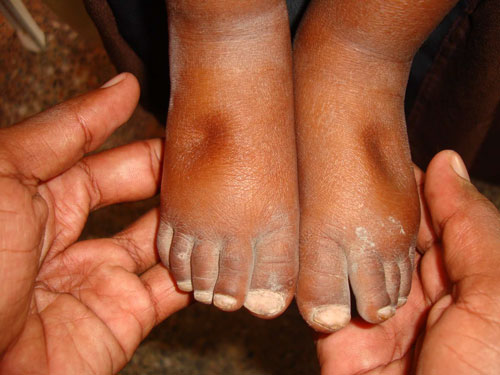
\includegraphics[width=6.94in]{images/oedemaStep2} 

}

\caption{Bilateral pitting oedema observed after releasing thumbs}\label{fig:oedemaStep2}
\end{figure}

\begin{enumerate}
\def\labelenumi{\arabic{enumi}.}
\setcounter{enumi}{2}
\item
  Move up to check on the lower legs If there is nutritional oedema
  present on the feet, perform the same test described in step 2 but now
  move up to the lower legs.
\item
  Move up to the upper body and/or face If there is nutritional oedema
  present on the lower legs, perform the same test described in step 2
  but now move up to the upper body and/or the face.
\end{enumerate}

\textbf{Step 3} and \textbf{Step 4} are performed to be able to grade or
classify the level of nutritional oedema the child is suffering from (if
present).

\begin{longtable}[]{@{}ll@{}}
\toprule
\begin{minipage}[b]{0.75\columnwidth}\raggedright
\textbf{Oedema Description}\strut
\end{minipage} & \begin{minipage}[b]{0.20\columnwidth}\raggedright
\textbf{Grade}\strut
\end{minipage}\tabularnewline
\midrule
\endhead
\begin{minipage}[t]{0.75\columnwidth}\raggedright
Oedema below the knees\strut
\end{minipage} & \begin{minipage}[t]{0.20\columnwidth}\raggedright
\texttt{+}\strut
\end{minipage}\tabularnewline
\begin{minipage}[t]{0.75\columnwidth}\raggedright
Oedema in both feet and legs, below the knees\strut
\end{minipage} & \begin{minipage}[t]{0.20\columnwidth}\raggedright
\texttt{++}\strut
\end{minipage}\tabularnewline
\begin{minipage}[t]{0.75\columnwidth}\raggedright
Oedema in both feet, legs, arms and sacral pad and eyelids\strut
\end{minipage} & \begin{minipage}[t]{0.20\columnwidth}\raggedright
\texttt{+++}\strut
\end{minipage}\tabularnewline
\bottomrule
\end{longtable}

\begin{enumerate}
\def\labelenumi{\arabic{enumi}.}
\setcounter{enumi}{4}
\tightlist
\item
  Record on the paper questionnaire or the mobile device the presence or
  absence of oedema. If oedema is present, record also the grade of the
  oedema.
\end{enumerate}

\BeginKnitrBlock{rmdnote}
Children with oedema (any grade) are at risk of dying and should be
immediately referred to a health care facility (ideally a facility that
manages severe acute undernutrition).
\EndKnitrBlock{rmdnote}

\BeginKnitrBlock{rmdremind}
\item 

Oedema is a very rare event.

\item 

It is the most common source of errors.

\item 

Be careful of misclassifying oedematous child.

\item 

Team leader and/or supervisor should confirm oedema.
\EndKnitrBlock{rmdremind}

\hypertarget{standard}{%
\chapter{Anthropometric measurement standardisation
test}\label{standard}}

The survey personnel should go through theoretical discussions and
demonstrations on how to perform the anthropometric measurements. This
should then be followed by practical demonstration of the measurement
techniques, measurement readings and recording ideally with a large
numbe of children particularly if there is a large number of survey
personnel. Once all personnel have had the opportunity to adequately
practice their measurement and recording techniques, a standardisation
test or exercise must be carried out. Chapter {[}\#standard{]} provides
detailed instructions on how to carry out an anthropometric measurement
standardisation test as part of a training process in preparation for a
nutrition survey.

\hypertarget{objectives}{%
\section{Objectives}\label{objectives}}

The standardisation test evaluates the \textbf{precision} and the
\textbf{accuracy} of the measurements taken by each survey personnel.

The \textbf{accuracy} of measurements taken by survey personnel is
determined by how close they are to the true value with repeated
measurements. On the other hand, the \textbf{precision} of measurements
taken by survey personnel is determined by how similar the values are of
repeated measurements made. In preparation for a nutrition survey while
the survey personnel are in training, the aim is for survey personnel to
be \emph{highly accurate} and \emph{highly precise} with their
anthropometric measurements.

\begin{figure}

{\centering 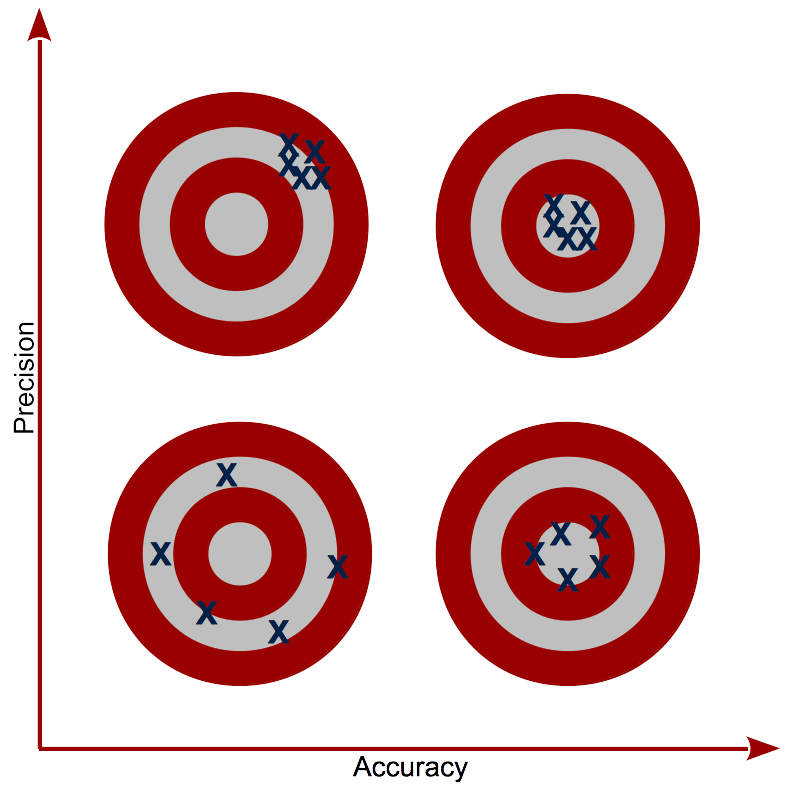
\includegraphics[width=11.11in]{images/accuracyPrecision} 

}

\caption{Relationship between accuracy and precision}\label{fig:standard01}
\end{figure}

\hypertarget{mechanics}{%
\section{Mechanics}\label{mechanics}}

The general process of the standardisation test is for each survey
personnel to take measurements of at least 10 children 6-59 months,
twice, with an interval of time between the 1st and 2nd measurements.

\hypertarget{test-parameters}{%
\subsection{Test parameters}\label{test-parameters}}

The following test parameters need to be followed when conducting an
anthopometric standardisation test:

\begin{enumerate}
\def\labelenumi{\arabic{enumi}.}
\item
  The same type of equipment must be used both during the
  standardisation test and the survey
\item
  Each child is measured with the same equipment
\item
  The supervisor must observe how measurements are being taken
\item
  Survey personnel measurements are compared to the reference
  (supervisor) values
\item
  Survey personnel measurements are compared to the repeated measures
  taken (intra-observer)
\end{enumerate}

\hypertarget{test-organisation-and-requirements}{%
\subsection{Test organisation and
requirements}\label{test-organisation-and-requirements}}

The following test organisation and requirements need to be met in order
to conduct a credible standardisation test:

\begin{enumerate}
\def\labelenumi{\arabic{enumi}.}
\item
  Spacious and shady area
\item
  Healthy children between 6 and 59 months or according to the age group
  targeted by the survey
\item
  Incentives provided for the mother and children
\item
  Survey personnel are grouped into pairs, but each personnel will carry
  out the measurements in turn
\item
  There should only be one pair of survey personnel per child at any
  time during the test
\item
  Each survey personnel is given a unique ID. For example if there are
  20 survey personnel, a unique ID from 1 to 20 is given to each survey
  personnel. The supervisor's ID is always 0
\item
  Each measurement station should have a height board, weighing scale
  and a MUAC tape
\item
  Each child must remain with their mother in a fixed station with a
  unique ID number. For example if there are 10 mother and children
  pairs, a unique ID from 1 to 10 is given to each pair
\item
  It is not allowed for pairs of survey personnel to speak with other
  pairs during the test
\end{enumerate}

\hypertarget{timeframe}{%
\subsection{Timeframe}\label{timeframe}}

In order to follow the test parameters specified above and organise the
test appropriately, a considerable amount of time needs to be set aside
for conducting the test.

For a survey team of about 20 survey personnel, the test can be carried
out in 2 half-days such that half of the survey personnel (first half of
each team) measures 10 children in the morning and the other half
(second half of each team) measures the same 10 children in the
afternoon.

It would be possible to have a different set of 10 children for the
afternoon session. However, the results of the first half who took the
test in the morning cannot be combined with the results of the second
half who took the test in the afternoon.

For larger scale surveys with survey personnel more than 20, more days
will be required to conduct the test to appropriately and to correct
specifiations.

\hypertarget{steps-in-carrying-out-the-standardisation-test}{%
\subsection{Steps in carrying out the standardisation
test}\label{steps-in-carrying-out-the-standardisation-test}}

\begin{enumerate}
\def\labelenumi{\arabic{enumi}.}
\tightlist
\item
  The supervisor carefully performs the measurements on each child
  without allowing the teams to see the values. The supervisor records
  his/her measurements on the standardisation test form for the first
  round of measurements.
\end{enumerate}

Standardisation Test Form - Measurement Round 1

Enumerator ID: \_\_\_\_\_ ~ ~ ~ Enumerator Name:
\_\_\_\_\_\_\_\_\_\_\_\_\_\_\_\_\_\_\_

\begin{longtable}[]{@{}lllll@{}}
\toprule
\begin{minipage}[b]{0.17\columnwidth}\raggedright
Child ID\strut
\end{minipage} & \begin{minipage}[b]{0.17\columnwidth}\raggedright
Weight (kg)\strut
\end{minipage} & \begin{minipage}[b]{0.17\columnwidth}\raggedright
Height (cm)\strut
\end{minipage} & \begin{minipage}[b]{0.17\columnwidth}\raggedright
MUAC (mm)\strut
\end{minipage} & \begin{minipage}[b]{0.17\columnwidth}\raggedright
Oedema (yes/no)\strut
\end{minipage}\tabularnewline
\midrule
\endhead
\begin{minipage}[t]{0.17\columnwidth}\raggedright
01\strut
\end{minipage} & \begin{minipage}[t]{0.17\columnwidth}\raggedright
\strut
\end{minipage} & \begin{minipage}[t]{0.17\columnwidth}\raggedright
\strut
\end{minipage} & \begin{minipage}[t]{0.17\columnwidth}\raggedright
\strut
\end{minipage} & \begin{minipage}[t]{0.17\columnwidth}\raggedright
\strut
\end{minipage}\tabularnewline
\begin{minipage}[t]{0.17\columnwidth}\raggedright
02\strut
\end{minipage} & \begin{minipage}[t]{0.17\columnwidth}\raggedright
\strut
\end{minipage} & \begin{minipage}[t]{0.17\columnwidth}\raggedright
\strut
\end{minipage} & \begin{minipage}[t]{0.17\columnwidth}\raggedright
\strut
\end{minipage} & \begin{minipage}[t]{0.17\columnwidth}\raggedright
\strut
\end{minipage}\tabularnewline
\begin{minipage}[t]{0.17\columnwidth}\raggedright
03\strut
\end{minipage} & \begin{minipage}[t]{0.17\columnwidth}\raggedright
\strut
\end{minipage} & \begin{minipage}[t]{0.17\columnwidth}\raggedright
\strut
\end{minipage} & \begin{minipage}[t]{0.17\columnwidth}\raggedright
\strut
\end{minipage} & \begin{minipage}[t]{0.17\columnwidth}\raggedright
\strut
\end{minipage}\tabularnewline
\begin{minipage}[t]{0.17\columnwidth}\raggedright
04\strut
\end{minipage} & \begin{minipage}[t]{0.17\columnwidth}\raggedright
\strut
\end{minipage} & \begin{minipage}[t]{0.17\columnwidth}\raggedright
\strut
\end{minipage} & \begin{minipage}[t]{0.17\columnwidth}\raggedright
\strut
\end{minipage} & \begin{minipage}[t]{0.17\columnwidth}\raggedright
\strut
\end{minipage}\tabularnewline
\begin{minipage}[t]{0.17\columnwidth}\raggedright
05\strut
\end{minipage} & \begin{minipage}[t]{0.17\columnwidth}\raggedright
\strut
\end{minipage} & \begin{minipage}[t]{0.17\columnwidth}\raggedright
\strut
\end{minipage} & \begin{minipage}[t]{0.17\columnwidth}\raggedright
\strut
\end{minipage} & \begin{minipage}[t]{0.17\columnwidth}\raggedright
\strut
\end{minipage}\tabularnewline
\begin{minipage}[t]{0.17\columnwidth}\raggedright
06\strut
\end{minipage} & \begin{minipage}[t]{0.17\columnwidth}\raggedright
\strut
\end{minipage} & \begin{minipage}[t]{0.17\columnwidth}\raggedright
\strut
\end{minipage} & \begin{minipage}[t]{0.17\columnwidth}\raggedright
\strut
\end{minipage} & \begin{minipage}[t]{0.17\columnwidth}\raggedright
\strut
\end{minipage}\tabularnewline
\begin{minipage}[t]{0.17\columnwidth}\raggedright
07\strut
\end{minipage} & \begin{minipage}[t]{0.17\columnwidth}\raggedright
\strut
\end{minipage} & \begin{minipage}[t]{0.17\columnwidth}\raggedright
\strut
\end{minipage} & \begin{minipage}[t]{0.17\columnwidth}\raggedright
\strut
\end{minipage} & \begin{minipage}[t]{0.17\columnwidth}\raggedright
\strut
\end{minipage}\tabularnewline
\begin{minipage}[t]{0.17\columnwidth}\raggedright
08\strut
\end{minipage} & \begin{minipage}[t]{0.17\columnwidth}\raggedright
\strut
\end{minipage} & \begin{minipage}[t]{0.17\columnwidth}\raggedright
\strut
\end{minipage} & \begin{minipage}[t]{0.17\columnwidth}\raggedright
\strut
\end{minipage} & \begin{minipage}[t]{0.17\columnwidth}\raggedright
\strut
\end{minipage}\tabularnewline
\begin{minipage}[t]{0.17\columnwidth}\raggedright
09\strut
\end{minipage} & \begin{minipage}[t]{0.17\columnwidth}\raggedright
\strut
\end{minipage} & \begin{minipage}[t]{0.17\columnwidth}\raggedright
\strut
\end{minipage} & \begin{minipage}[t]{0.17\columnwidth}\raggedright
\strut
\end{minipage} & \begin{minipage}[t]{0.17\columnwidth}\raggedright
\strut
\end{minipage}\tabularnewline
\begin{minipage}[t]{0.17\columnwidth}\raggedright
10\strut
\end{minipage} & \begin{minipage}[t]{0.17\columnwidth}\raggedright
\strut
\end{minipage} & \begin{minipage}[t]{0.17\columnwidth}\raggedright
\strut
\end{minipage} & \begin{minipage}[t]{0.17\columnwidth}\raggedright
\strut
\end{minipage} & \begin{minipage}[t]{0.17\columnwidth}\raggedright
\strut
\end{minipage}\tabularnewline
\bottomrule
\end{longtable}

\BeginKnitrBlock{rmddownload}
Download the standardisation test form
\href{pdf/standardForm.pdf}{here}.
\EndKnitrBlock{rmddownload}

\begin{enumerate}
\def\labelenumi{\arabic{enumi}.}
\setcounter{enumi}{1}
\item
  Each team starts with a different child, and the first half of the
  team measures the child once and records the results in a standard
  form for the 1st measurement (as above). The current measurer should
  make sure that he/she is entering data in the row corresponding to the
  child ID of the child he/she is currently measuring.
\item
  When the first half of the team has done the measurements for the
  current child, they should move on to the next child. After the first
  half of all the teams has measured 10 children once, the first
  measurement round forms are handed in. The teams and the children then
  take a break. Appropriate incentives including food and drinks to
  snack on during the break should be provided to the mothers and
  children.
\item
  After the break, the first half of the team repeats the whole process
  and measures each child for the second time and records his/her
  measurements onto the standardisation test form for the second round
  of measurements. After the the first half of all the teams has
  measured 10 children twice, the second measurement round forms are
  handed in. The teams and the children then take a break for lunch (end
  of first half of the day/first half of the test). Appropriate lunch
  arrangements should be prepared for the mothers and children.
\item
  After the lunch break or on a new day altogether, the whole process is
  done all over again but this time, the second half of the teams will
  be performing the measurements. Ideally, the same set of mother and
  child pairs should be utilised for the second half day of testing.
  However, it may be that some of the mothers will be unable to come
  back to help. If for the second half day of testing the mother and
  child pairs are different from the first half day, then measurements
  made in the second half day cannot be mixed with the data from the
  first half day when reporting on the performance in the
  standardisation test of the survey personnel.
\end{enumerate}

\hypertarget{diet}{%
\chapter{Measuring dietary diversity}\label{diet}}

\hypertarget{introduction-1}{%
\section{Introduction}\label{introduction-1}}

Dietary diversity can be measured in various ways with the traditional
approach being time consuming, expensive, and requiring a high level of
technical skill both in data collection and analysis. Recent development
work in this indicator has brought about the use of a qualitative
approach to food consumption that reflects household access to a wide
variety of foods, and is also a proxy of the nutrient adequacy of the
diet for individuals. The approach uses a specifically designed and
tested dietary diversity questionnaire as a tool to elicit food
consumption information in a more rapid, user-friendly and
cost-effective approach. Administration of the questionnaire is
straightforward and can be handled easily by trained enumerators. The
scoring and/or analysis of the information gained from the questionnaire
is easy to understand, quick to implement, and can be applied with
minimal technical expertise.

In general, dietary diversity indicators are created by summing either
the number of individual foods or food groups consumed over a reference
period. This \protect\hyperlink{diet}{chapter} describes how an
individual dietary diversity indicator is created through a simple count
of food groups that an individual has consumed over the past 24 hours.
Specifically, this \protect\hyperlink{diet}{chapter} discusses how the
minimum dietary diversity indicator for women (MDD-W) and the minimum
dietary diversity indicator for children under 2 years old (MDD) are
calculated using a standard dietary diversity questionnaire.

\hypertarget{minimum-dietary-diversity-for-women-mdd-w}{%
\section{Minimum dietary diversity for women
(MDD-W)}\label{minimum-dietary-diversity-for-women-mdd-w}}

MDD-W is a dichotomous indicator of whether or not women 15--49 years of
age have consumed at least five out of ten defined food groups the
previous day or night. The proportion of women 15--49 years of age who
reach this minimum in a population can be used as a proxy indicator for
higher micronutrient adequacy, one important dimension of diet quality.

The indicator is calculated as follows:

\[ \text{MDD-W} = \frac{\text{Women 15-49 years of age who consumed 5 out of 10 food groups in the previous day or night}}{\text{Women 15-49 years of age}} \]

The ten food groups are:

\begin{enumerate}
\def\labelenumi{\arabic{enumi}.}
\tightlist
\item
  Grains, white roots and tubers, and plantains
\item
  Pulses (beans, peas and lentils)
\item
  Nuts and seeds
\item
  Dairy
\item
  Meat, poultry and fish
\item
  Eggs
\item
  Dark green leafy vegetables
\item
  Other vitamin A-rich fruits and vegetables
\item
  Other vegetables
\item
  Other fruits
\end{enumerate}

\hypertarget{mdd-w-questionnaire}{%
\subsection{MDD-W questionnaire}\label{mdd-w-questionnaire}}

The following is a model questionnaire used for eliciting dietary
diversity information from a women 15-49 years old.

\textbf{1. Following are required elements of the questionnaire}

\begin{longtable}[]{@{}clll@{}}
\toprule
\begin{minipage}[b]{0.05\columnwidth}\centering
\strut
\end{minipage} & \begin{minipage}[b]{0.18\columnwidth}\raggedright
\textbf{Food categories}\strut
\end{minipage} & \begin{minipage}[b]{0.54\columnwidth}\raggedright
\textbf{Description and/or examples (to be adapted to local
context)}\strut
\end{minipage} & \begin{minipage}[b]{0.12\columnwidth}\raggedright
\textbf{Consumed?}\strut
\end{minipage}\tabularnewline
\midrule
\endhead
\begin{minipage}[t]{0.05\columnwidth}\centering
A\strut
\end{minipage} & \begin{minipage}[t]{0.18\columnwidth}\raggedright
Food made from grains\strut
\end{minipage} & \begin{minipage}[t]{0.54\columnwidth}\raggedright
Porridge, bread, rice, pasta/noodles or other foods made from
grains\strut
\end{minipage} & \begin{minipage}[t]{0.12\columnwidth}\raggedright
Yes = 1 No = 2\strut
\end{minipage}\tabularnewline
\begin{minipage}[t]{0.05\columnwidth}\centering
B\strut
\end{minipage} & \begin{minipage}[t]{0.18\columnwidth}\raggedright
White roots and tubers\strut
\end{minipage} & \begin{minipage}[t]{0.54\columnwidth}\raggedright
White potatoes, white yams, manioc/cassava/yucca, cocoyam, taro or any
other foods made from white- eshed roots or tubers, or plantains\strut
\end{minipage} & \begin{minipage}[t]{0.12\columnwidth}\raggedright
Yes = 1 No = 2\strut
\end{minipage}\tabularnewline
\begin{minipage}[t]{0.05\columnwidth}\centering
C\strut
\end{minipage} & \begin{minipage}[t]{0.18\columnwidth}\raggedright
Pulses (beans, peas and lentils)\strut
\end{minipage} & \begin{minipage}[t]{0.54\columnwidth}\raggedright
Mature beans or peas (fresh or dried seed), len ls or bean/pea products,
including hummus, tofu and tempeh\strut
\end{minipage} & \begin{minipage}[t]{0.12\columnwidth}\raggedright
Yes = 1 No = 2\strut
\end{minipage}\tabularnewline
\begin{minipage}[t]{0.05\columnwidth}\centering
D\strut
\end{minipage} & \begin{minipage}[t]{0.18\columnwidth}\raggedright
Nuts and seeds\strut
\end{minipage} & \begin{minipage}[t]{0.54\columnwidth}\raggedright
Any tree nut, groundnut/peanut or certain seeds, or nut/seed ``butters''
or pastes\strut
\end{minipage} & \begin{minipage}[t]{0.12\columnwidth}\raggedright
Yes = 1 No = 2\strut
\end{minipage}\tabularnewline
\begin{minipage}[t]{0.05\columnwidth}\centering
E\strut
\end{minipage} & \begin{minipage}[t]{0.18\columnwidth}\raggedright
Milk and milk products\strut
\end{minipage} & \begin{minipage}[t]{0.54\columnwidth}\raggedright
Milk, cheese, yoghurt or other milk products but NOT including butter,
ice cream, cream or sour cream\strut
\end{minipage} & \begin{minipage}[t]{0.12\columnwidth}\raggedright
Yes = 1 No = 2\strut
\end{minipage}\tabularnewline
\begin{minipage}[t]{0.05\columnwidth}\centering
F\strut
\end{minipage} & \begin{minipage}[t]{0.18\columnwidth}\raggedright
Organ meat\strut
\end{minipage} & \begin{minipage}[t]{0.54\columnwidth}\raggedright
Liver, kidney, heart or other organ meats or blood-based foods,
including from wild game\strut
\end{minipage} & \begin{minipage}[t]{0.12\columnwidth}\raggedright
Yes = 1 No = 2\strut
\end{minipage}\tabularnewline
\begin{minipage}[t]{0.05\columnwidth}\centering
G\strut
\end{minipage} & \begin{minipage}[t]{0.18\columnwidth}\raggedright
Meat and poultry\strut
\end{minipage} & \begin{minipage}[t]{0.54\columnwidth}\raggedright
Beef, pork, lamb, goat, rabbit, wild game meat, chicken, duck or other
bird\strut
\end{minipage} & \begin{minipage}[t]{0.12\columnwidth}\raggedright
Yes = 1 No = 2\strut
\end{minipage}\tabularnewline
\begin{minipage}[t]{0.05\columnwidth}\centering
H\strut
\end{minipage} & \begin{minipage}[t]{0.18\columnwidth}\raggedright
Fish and seafood\strut
\end{minipage} & \begin{minipage}[t]{0.54\columnwidth}\raggedright
Fresh or dried fish, shellfish or seafood\strut
\end{minipage} & \begin{minipage}[t]{0.12\columnwidth}\raggedright
Yes = 1 No = 2\strut
\end{minipage}\tabularnewline
\begin{minipage}[t]{0.05\columnwidth}\centering
I\strut
\end{minipage} & \begin{minipage}[t]{0.18\columnwidth}\raggedright
Eggs\strut
\end{minipage} & \begin{minipage}[t]{0.54\columnwidth}\raggedright
Eggs from poultry or any other bird\strut
\end{minipage} & \begin{minipage}[t]{0.12\columnwidth}\raggedright
Yes = 1 No = 2\strut
\end{minipage}\tabularnewline
\begin{minipage}[t]{0.05\columnwidth}\centering
J\strut
\end{minipage} & \begin{minipage}[t]{0.18\columnwidth}\raggedright
Dark green leafy vegetables\strut
\end{minipage} & \begin{minipage}[t]{0.54\columnwidth}\raggedright
List examples of any medium-to-dark green leafy vegetables, including
wild/foraged leaves\strut
\end{minipage} & \begin{minipage}[t]{0.12\columnwidth}\raggedright
Yes = 1 No = 2\strut
\end{minipage}\tabularnewline
\begin{minipage}[t]{0.05\columnwidth}\centering
K\strut
\end{minipage} & \begin{minipage}[t]{0.18\columnwidth}\raggedright
Vitamin A-rich vegetables, roots and tubers\strut
\end{minipage} & \begin{minipage}[t]{0.54\columnwidth}\raggedright
Pumpkin, carrots, squash or sweet potatoes that are yellow or orange
inside\strut
\end{minipage} & \begin{minipage}[t]{0.12\columnwidth}\raggedright
Yes = 1 No = 2\strut
\end{minipage}\tabularnewline
\begin{minipage}[t]{0.05\columnwidth}\centering
L\strut
\end{minipage} & \begin{minipage}[t]{0.18\columnwidth}\raggedright
Vitamin A-rich fruits\strut
\end{minipage} & \begin{minipage}[t]{0.54\columnwidth}\raggedright
Ripe mango, ripe papaya, some melons\strut
\end{minipage} & \begin{minipage}[t]{0.12\columnwidth}\raggedright
Yes = 1 No = 2\strut
\end{minipage}\tabularnewline
\begin{minipage}[t]{0.05\columnwidth}\centering
M\strut
\end{minipage} & \begin{minipage}[t]{0.18\columnwidth}\raggedright
Other vegetables\strut
\end{minipage} & \begin{minipage}[t]{0.54\columnwidth}\raggedright
List examples of any other vegetables\strut
\end{minipage} & \begin{minipage}[t]{0.12\columnwidth}\raggedright
Yes = 1 No = 2\strut
\end{minipage}\tabularnewline
\begin{minipage}[t]{0.05\columnwidth}\centering
N\strut
\end{minipage} & \begin{minipage}[t]{0.18\columnwidth}\raggedright
Other fruits\strut
\end{minipage} & \begin{minipage}[t]{0.54\columnwidth}\raggedright
List examples of any other fruits\strut
\end{minipage} & \begin{minipage}[t]{0.12\columnwidth}\raggedright
Yes = 1 No = 2\strut
\end{minipage}\tabularnewline
\bottomrule
\end{longtable}

\textbf{2. Optional components of the questionnaire}

\begin{longtable}[]{@{}clll@{}}
\toprule
\begin{minipage}[b]{0.05\columnwidth}\centering
\strut
\end{minipage} & \begin{minipage}[b]{0.18\columnwidth}\raggedright
\textbf{Food categories}\strut
\end{minipage} & \begin{minipage}[b]{0.54\columnwidth}\raggedright
\textbf{Description and/or examples (to be adapted to local
context)}\strut
\end{minipage} & \begin{minipage}[b]{0.12\columnwidth}\raggedright
\textbf{Consumed?}\strut
\end{minipage}\tabularnewline
\midrule
\endhead
\begin{minipage}[t]{0.05\columnwidth}\centering
O\strut
\end{minipage} & \begin{minipage}[t]{0.18\columnwidth}\raggedright
Insects and other small protein foods\strut
\end{minipage} & \begin{minipage}[t]{0.54\columnwidth}\raggedright
Insects, insect larvae/grubs, insect eggs and land and sea snails\strut
\end{minipage} & \begin{minipage}[t]{0.12\columnwidth}\raggedright
Yes = 1 No = 2\strut
\end{minipage}\tabularnewline
\begin{minipage}[t]{0.05\columnwidth}\centering
P\strut
\end{minipage} & \begin{minipage}[t]{0.18\columnwidth}\raggedright
Red palm oil\strut
\end{minipage} & \begin{minipage}[t]{0.54\columnwidth}\raggedright
Red palm oil\strut
\end{minipage} & \begin{minipage}[t]{0.12\columnwidth}\raggedright
Yes = 1 No = 2\strut
\end{minipage}\tabularnewline
\begin{minipage}[t]{0.05\columnwidth}\centering
Q\strut
\end{minipage} & \begin{minipage}[t]{0.18\columnwidth}\raggedright
Other oils and fats\strut
\end{minipage} & \begin{minipage}[t]{0.54\columnwidth}\raggedright
Oil; fats or bu er added to food or used for cooking, including
extracted oils from nuts, fruits and seeds; and all animal fat\strut
\end{minipage} & \begin{minipage}[t]{0.12\columnwidth}\raggedright
Yes = 1 No = 2\strut
\end{minipage}\tabularnewline
\begin{minipage}[t]{0.05\columnwidth}\centering
R\strut
\end{minipage} & \begin{minipage}[t]{0.18\columnwidth}\raggedright
Savoury and fried snacks\strut
\end{minipage} & \begin{minipage}[t]{0.54\columnwidth}\raggedright
Crisps and chips, fried dough or other fried snacks\strut
\end{minipage} & \begin{minipage}[t]{0.12\columnwidth}\raggedright
Yes = 1 No = 2\strut
\end{minipage}\tabularnewline
\begin{minipage}[t]{0.05\columnwidth}\centering
S\strut
\end{minipage} & \begin{minipage}[t]{0.18\columnwidth}\raggedright
Sweets\strut
\end{minipage} & \begin{minipage}[t]{0.54\columnwidth}\raggedright
Sugary foods, such as chocolates, candies, cookies/sweet biscuits and
cakes, sweet pastries or ice cream\strut
\end{minipage} & \begin{minipage}[t]{0.12\columnwidth}\raggedright
Yes = 1 No = 2\strut
\end{minipage}\tabularnewline
\begin{minipage}[t]{0.05\columnwidth}\centering
T\strut
\end{minipage} & \begin{minipage}[t]{0.18\columnwidth}\raggedright
Sugar-sweetened beverages\strut
\end{minipage} & \begin{minipage}[t]{0.54\columnwidth}\raggedright
Sweetened fruit juices and ``juice drinks'', softdrinks/fizzy drinks,
chocolate drinks, malt drinks, yoghurt drinks or sweet tea or coffee
with sugar\strut
\end{minipage} & \begin{minipage}[t]{0.12\columnwidth}\raggedright
Yes = 1 No = 2\strut
\end{minipage}\tabularnewline
\bottomrule
\end{longtable}

\textbf{3. Other required components of the questionniare but don't
count in the food groups}

\begin{longtable}[]{@{}clll@{}}
\toprule
\begin{minipage}[b]{0.05\columnwidth}\centering
\strut
\end{minipage} & \begin{minipage}[b]{0.18\columnwidth}\raggedright
\textbf{Food categories}\strut
\end{minipage} & \begin{minipage}[b]{0.54\columnwidth}\raggedright
\textbf{Description and/or examples (to be adapted to local
context)}\strut
\end{minipage} & \begin{minipage}[b]{0.12\columnwidth}\raggedright
\textbf{Consumed?}\strut
\end{minipage}\tabularnewline
\midrule
\endhead
\begin{minipage}[t]{0.05\columnwidth}\centering
U\strut
\end{minipage} & \begin{minipage}[t]{0.18\columnwidth}\raggedright
Condiments and seasonings\strut
\end{minipage} & \begin{minipage}[t]{0.54\columnwidth}\raggedright
Ingredients used in small quan es for avour, such as chilies, spices,
herbs, sh powder, tomato paste, avour cubes or seeds\strut
\end{minipage} & \begin{minipage}[t]{0.12\columnwidth}\raggedright
Yes = 1 No = 2\strut
\end{minipage}\tabularnewline
\begin{minipage}[t]{0.05\columnwidth}\centering
V\strut
\end{minipage} & \begin{minipage}[t]{0.18\columnwidth}\raggedright
Other beverages and foods (optionally, specify if not listed)\strut
\end{minipage} & \begin{minipage}[t]{0.54\columnwidth}\raggedright
Tea or co ee if not sweetened, clear broth, alcohol Pickles, olives and
similar\strut
\end{minipage} & \begin{minipage}[t]{0.12\columnwidth}\raggedright
Yes = 1 No = 2\strut
\end{minipage}\tabularnewline
\bottomrule
\end{longtable}

\hypertarget{mdd-w-food-group-description}{%
\subsection{MDD-W food group
description}\label{mdd-w-food-group-description}}

\textbf{1. Grains, white roots and tubers, and plantains}

\begin{itemize}
\tightlist
\item
  Also called as ``starchy staples''"
\item
  Examples include

  \begin{itemize}
  \tightlist
  \item
    breads and flatbreads
  \item
    stiff porridges of maize, sorghum, millet or cassava (manioc)
  \item
    pasta
  \item
    potatoes
  \item
    white-fleshed sweet potatoes
  \item
    white yams
  \item
    yucca
  \item
    plantains (white-fleshed)
  \end{itemize}
\end{itemize}

\textbf{2. Pulses (beans, peas and lentils)}

\begin{itemize}
\tightlist
\item
  Beans, peas and lentils the seeds of which are dried and used as food
  for processed into other food products
\item
  Does not include the same plants eaten fresh in the pod or still
  green/immature (these are categorised as ``other vegetables'')
\item
  Groundnut (peanut), a legume, is not included in this group (these are
  categorised as ``nuts'')
\item
  Examples include

  \begin{itemize}
  \tightlist
  \item
    beans - black, kidney, pinto
  \item
    broad bean - fava, field bean
  \item
    chickpea (garbanzo)
  \item
    pigeon pea
  \item
    cowpea
  \item
    lentil and soybean/soybean products or other legume products
  \end{itemize}
\end{itemize}

\textbf{3. Nuts and seeds}

\begin{itemize}
\tightlist
\item
  Comprise mostly of tree nuts but also includes peanuts (groundnuts)
\item
  Certain seeds consumed in substantial quantities (otherwise
  categorised as ``condiments and seasonings'')
\item
  Includes nut and seed butters such as peanut butter, cashew butter or
  sesame butter (tahini)
\item
  Examples of nuts are

  \begin{itemize}
  \tightlist
  \item
    cashew
  \item
    macadamia
  \item
    Brazil nut
  \item
    almond
  \item
    chestnut
  \item
    hazelnut
  \item
    pistachio
  \item
    walnut
  \end{itemize}
\item
  Examples of seeds are

  \begin{itemize}
  \tightlist
  \item
    sesame
  \item
    sunflower
  \item
    pumpkin/squash/gourd
  \item
    pine nut
  \end{itemize}
\end{itemize}

\textbf{4. Dairy}

\begin{itemize}
\tightlist
\item
  Includes

  \begin{itemize}
  \tightlist
  \item
    Almost all liquid and solid dairy products from cows, goats,
    buffalo, sheep or camels.
  \item
    Tinned, powdered or ultra-high temperature (UHT) milk
  \item
    Soft and hard cheeses
  \item
    Yoghurt and kefir
  \end{itemize}
\item
  Excludes

  \begin{itemize}
  \tightlist
  \item
    Butter
  \item
    Cream
  \item
    Sour cream
  \item
    Ice cream
  \item
    Sweetened condensed milk
  \item
    Processed/packaged ``yoghurt drinks''
  \end{itemize}
\end{itemize}

\textbf{5. Meat, poultry and fish}

\begin{itemize}
\tightlist
\item
  Sometimes referred to as ``flesh foods''
\item
  All meats, organ meats, poultry and other birds
\item
  Fresh and dried fish and seafood/shellfish
\item
  Wild birds and mammals (``bush meat''),
\item
  Snakes, frogs and other reptiles and amphibians
\end{itemize}

\textbf{6. Eggs}

\begin{itemize}
\tightlist
\item
  Includes eggs from any type of bird (domesticated poultry and wild
  birds)
\item
  Excludes fish roe (categorised with small protein foods)
\end{itemize}

\textbf{7. Dark green leafy vegetables}

\begin{itemize}
\tightlist
\item
  All medium-to-dark green leafy vegetables
\item
  Only very light green leaves, such as iceberg lettuce, are not.
\item
  Medium green leaves, such as Chinese cabbage, romaine and bibb
  lettuce, along with darker greens are included
\item
  Dark green leafy vegetables that are wild and foraged
\item
  Dark green leafy vegetbles of other food crops such as cassava leaves,
  bean leaves, pumpkin leaves, amaranth leaves)
\end{itemize}

\textbf{8. Other vitamin A-rich fruits and vegetables}

\begin{itemize}
\tightlist
\item
  Vitamin A-rich fruits are

  \begin{itemize}
  \tightlist
  \item
    Ripe mango (not when eaten green; categorised as ``other fruits'')
  \item
    Ripe papaya (not when eaten green; categorised as ``other fruits'')
  \item
    Red palm fruit/pulp
  \item
    Passion fruit
  \item
    Apricot
  \item
    Several types of melon
  \item
    Ripe, deep yellow-fleshed or orange-fleshed bananas (distinguish
    from white-fleshed bananas)
  \end{itemize}
\item
  Vitamin A-rich vegetables

  \begin{itemize}
  \tightlist
  \item
    Orange-fleshed sweet potato (if white-fleshed, categorised as roots
    and tubers)
  \item
    Carrot
  \item
    Pumpkin
  \item
    Deep yellow or orange-fleshed squash
  \end{itemize}
\end{itemize}

\textbf{9. Other vegetables}

\begin{itemize}
\tightlist
\item
  Includes legumes when the fresh/green pod is consumed (as in fresh
  peas, snow peas, snap peas or green beans)
\item
  Includes stems, fruits and owers of plants when generally consumed in
  savoury dishes and considered as vegetables in culinary systems such
  as cucumber, tomato and okra
\item
  Excludes white potatoes, white yams, cassava and cocoyam
\end{itemize}

\textbf{10. Other fruits}

\begin{itemize}
\tightlist
\item
  Includes most fruits, excluding vitamin A-rich fruits
\item
  Does not include tomatoes
\item
  Plantains are classified with starchy staples but sweet white bananas
  are classified with fruit.
\end{itemize}

\hypertarget{minimum-dietary-diversity-mdd-component-of-the-infant-and-young-child-feeding-iycf}{%
\section{Minimum dietary diversity (MDD) component of the infant and
young child feeding
(IYCF)}\label{minimum-dietary-diversity-mdd-component-of-the-infant-and-young-child-feeding-iycf}}

MDD component of the IYCF indicators is a dichotomous indicator of
whether or not children 6-23 months of age receive foods from 4 or more
food groups (out of a total of 7 food groups for children). The
proportion of children 6--23 months of age who receive foods from 4 or
more food groups is associated with better quality diets for both
breastfed and non-breastfed children. Consumption of foods from at least
4 food groups on the previous day would mean that in most populations
the child had a high likelihood of consuming at least one animal-source
food and at least one fruit or vegetable that day, in addition to a
staple food (grain, root or tuber).

The indicator is calculated as follows:

\[ \text{MDD} = \frac{\text{Children 6–23 months of age who received foods from ≥ 4 food groups during the previous day}}{\text{Children 6–23 months of age}} \]

The 7 foods groups used for tabulation of this indicator are:

\begin{enumerate}
\def\labelenumi{\arabic{enumi}.}
\tightlist
\item
  Grains, roots and tubers
\item
  Legumes and nuts
\item
  Dairy products (milk, yogurt, cheese)
\item
  Fresh foods (meat, fish, poultry and liver/organ meats)
\item
  Eggs
\item
  Vitamin-A rich fruits and vegetables
\item
  Other fruits and vegetables
\end{enumerate}

Consumption of any amount of food from each food group is suf cient to
``count'', i.e., there is no minimum quantity, except if an item is only
used as a condiment.

\hypertarget{mdd-questionnaire}{%
\subsection{MDD questionnaire}\label{mdd-questionnaire}}

Following is a model questionnaire used for MDD component of IYCF

\begin{longtable}[]{@{}cll@{}}
\toprule
\begin{minipage}[b]{0.06\columnwidth}\centering
\strut
\end{minipage} & \begin{minipage}[b]{0.68\columnwidth}\raggedright
\textbf{Questions and filters}\strut
\end{minipage} & \begin{minipage}[b]{0.18\columnwidth}\raggedright
\textbf{Response}\strut
\end{minipage}\tabularnewline
\midrule
\endhead
\begin{minipage}[t]{0.06\columnwidth}\centering
A\strut
\end{minipage} & \begin{minipage}[t]{0.68\columnwidth}\raggedright
Porridge, bread, rice, noodles, or other foods made from grains\strut
\end{minipage} & \begin{minipage}[t]{0.18\columnwidth}\raggedright
Yes = 1 No = 2\strut
\end{minipage}\tabularnewline
\begin{minipage}[t]{0.06\columnwidth}\centering
B\strut
\end{minipage} & \begin{minipage}[t]{0.68\columnwidth}\raggedright
Pumpkin, carrots, squash, or sweet potatoes that are yellow or orange
inside\strut
\end{minipage} & \begin{minipage}[t]{0.18\columnwidth}\raggedright
Yes = 1 No = 2\strut
\end{minipage}\tabularnewline
\begin{minipage}[t]{0.06\columnwidth}\centering
C\strut
\end{minipage} & \begin{minipage}[t]{0.68\columnwidth}\raggedright
White potatoes, white yams, manioc, cassava, or any other foods made
from roots\strut
\end{minipage} & \begin{minipage}[t]{0.18\columnwidth}\raggedright
Yes = 1 No = 2\strut
\end{minipage}\tabularnewline
\begin{minipage}[t]{0.06\columnwidth}\centering
D\strut
\end{minipage} & \begin{minipage}[t]{0.68\columnwidth}\raggedright
Any dark green leafy vegetables\strut
\end{minipage} & \begin{minipage}[t]{0.18\columnwidth}\raggedright
Yes = 1 No = 2\strut
\end{minipage}\tabularnewline
\begin{minipage}[t]{0.06\columnwidth}\centering
E\strut
\end{minipage} & \begin{minipage}[t]{0.68\columnwidth}\raggedright
Ripe mangoes, ripe papayas, or (insert other local vitamin A-rich
fruits)\strut
\end{minipage} & \begin{minipage}[t]{0.18\columnwidth}\raggedright
Yes = 1 No = 2\strut
\end{minipage}\tabularnewline
\begin{minipage}[t]{0.06\columnwidth}\centering
F\strut
\end{minipage} & \begin{minipage}[t]{0.68\columnwidth}\raggedright
Any other fruits or vegetables\strut
\end{minipage} & \begin{minipage}[t]{0.18\columnwidth}\raggedright
Yes = 1 No = 2\strut
\end{minipage}\tabularnewline
\begin{minipage}[t]{0.06\columnwidth}\centering
G\strut
\end{minipage} & \begin{minipage}[t]{0.68\columnwidth}\raggedright
Liver, kidney, heart, or other organ meats\strut
\end{minipage} & \begin{minipage}[t]{0.18\columnwidth}\raggedright
Yes = 1 No = 2\strut
\end{minipage}\tabularnewline
\begin{minipage}[t]{0.06\columnwidth}\centering
H\strut
\end{minipage} & \begin{minipage}[t]{0.68\columnwidth}\raggedright
Any meat, such as beef, pork, lamb, goat, chicken, or duck\strut
\end{minipage} & \begin{minipage}[t]{0.18\columnwidth}\raggedright
Yes = 1 No = 2\strut
\end{minipage}\tabularnewline
\begin{minipage}[t]{0.06\columnwidth}\centering
I\strut
\end{minipage} & \begin{minipage}[t]{0.68\columnwidth}\raggedright
Eggs\strut
\end{minipage} & \begin{minipage}[t]{0.18\columnwidth}\raggedright
Yes = 1 No = 2\strut
\end{minipage}\tabularnewline
\begin{minipage}[t]{0.06\columnwidth}\centering
J\strut
\end{minipage} & \begin{minipage}[t]{0.68\columnwidth}\raggedright
Fresh or dried fish, shellfish, or seafood\strut
\end{minipage} & \begin{minipage}[t]{0.18\columnwidth}\raggedright
Yes = 1 No = 2\strut
\end{minipage}\tabularnewline
\begin{minipage}[t]{0.06\columnwidth}\centering
K\strut
\end{minipage} & \begin{minipage}[t]{0.68\columnwidth}\raggedright
Any foods made from beans, peas, lentils, nuts, or seeds\strut
\end{minipage} & \begin{minipage}[t]{0.18\columnwidth}\raggedright
Yes = 1 No = 2\strut
\end{minipage}\tabularnewline
\begin{minipage}[t]{0.06\columnwidth}\centering
L\strut
\end{minipage} & \begin{minipage}[t]{0.68\columnwidth}\raggedright
Cheese, yogurt, or other milk products\strut
\end{minipage} & \begin{minipage}[t]{0.18\columnwidth}\raggedright
Yes = 1 No = 2\strut
\end{minipage}\tabularnewline
\begin{minipage}[t]{0.06\columnwidth}\centering
M\strut
\end{minipage} & \begin{minipage}[t]{0.68\columnwidth}\raggedright
Any oil, fats, or butter, or foods made with any of these\strut
\end{minipage} & \begin{minipage}[t]{0.18\columnwidth}\raggedright
Yes = 1 No = 2\strut
\end{minipage}\tabularnewline
\begin{minipage}[t]{0.06\columnwidth}\centering
N\strut
\end{minipage} & \begin{minipage}[t]{0.68\columnwidth}\raggedright
Any sugary foods such as chocolates, sweets, candies, pastries, cakes,
or biscuits\strut
\end{minipage} & \begin{minipage}[t]{0.18\columnwidth}\raggedright
Yes = 1 No = 2 Yes = 1 No = 2\strut
\end{minipage}\tabularnewline
\begin{minipage}[t]{0.06\columnwidth}\centering
O\strut
\end{minipage} & \begin{minipage}[t]{0.68\columnwidth}\raggedright
Condiments for flavor, such as chilies, spices, herbs, or fish
powder\strut
\end{minipage} & \begin{minipage}[t]{0.18\columnwidth}\raggedright
Yes = 1 No = 2\strut
\end{minipage}\tabularnewline
\begin{minipage}[t]{0.06\columnwidth}\centering
P\strut
\end{minipage} & \begin{minipage}[t]{0.68\columnwidth}\raggedright
Grubs, snails, or insects\strut
\end{minipage} & \begin{minipage}[t]{0.18\columnwidth}\raggedright
Yes = 1 No = 2\strut
\end{minipage}\tabularnewline
\begin{minipage}[t]{0.06\columnwidth}\centering
Q\strut
\end{minipage} & \begin{minipage}[t]{0.68\columnwidth}\raggedright
Foods made with red palm oil, red palm nut, or red palm nut pulp
sauce\strut
\end{minipage} & \begin{minipage}[t]{0.18\columnwidth}\raggedright
Yes = 1 No = 2\strut
\end{minipage}\tabularnewline
\bottomrule
\end{longtable}

\hypertarget{mdd-food-group-description}{%
\subsection{MDD food group
description}\label{mdd-food-group-description}}

The food group description for MDD-W is about the same for the IYCF MDD
with a few exceptions:

\textbf{1. Ice cream}

In MDD-W, ice cream is categorised as ``sweets'' because it is a high
fat/high sugar food. For IYCF MDD, ice cream is categorised as dairy.

This difference is primarily due to increasing concerns with other
dimensions of diet quality in the context of the nutrition transition
given that ice cream is a high fat and high sugar food and also because
many low-quality ice cream products contain very little dairy.

\textbf{2. Garlic}

In MDD-W, garlic is categorised as ``condiments and seasonings'' given
that it is usually consumed in small quantities. In IYCF MDD, there is
no particular concern for food quantity so garlic is categorised as
``other fruits and vegetables''.

\textbf{3. Olives}

In MDD-W, olives are categorised as ``other foods and beverages'' given
that it is usually consumed in small quantities. In IYCF MDD, olives are
categorised as ``other fruits and vegetables''.

\textbf{4. Red palm oil}

In MDD-W, this is totally excluded from the indicator calculation. In
IYCF MDD, it is counted under ``vitamin A-rich fruits and vegetables''

\textbf{5. Fish roe}

In MDD-W, categorised with ``insects and other small protein foods''. In
IYCF MDD, categorised under ``fish and seafood''

\textbf{6. Seaweed}

In MDD-W, categorised as ``other vegetables''. In IYCF MDD, categorised
as ``dark green leafy vegetables''.

\hypertarget{food}{%
\chapter{Measuring food consumption}\label{food}}

\hypertarget{introduction-2}{%
\section{Introduction}\label{introduction-2}}

The \textbf{Food Consumption Score (FCS)} is an index developed by the
World Food Programme (WFP) in 1996. The \textbf{FCS} is a household
level indicator that aggregates food group diversity and frequency over
the past 7 days. These food groups are then weighted according to their
relative nutritional value. This means that food groups that are
nutritionally-dense such as animal products are given greater weight
than those containing less nutritionally dense foods such as tubers. The
weights are then added up to come up with a household score which are
then used to classify households into either poor, borderline, or
acceptable food consumption. The \textbf{FCS} is a measure of quantity
of caloric intake.

\hypertarget{fcs-questionnaire}{%
\section{FCS questionnaire}\label{fcs-questionnaire}}

A brief questionnaire is used to ask respondents about the frequency of
their households' consumption of eight different food groups over the
previous seven days. The eight food groups are:

\begin{enumerate}
\def\labelenumi{\arabic{enumi}.}
\tightlist
\item
  Main staples
\item
  Pulses
\item
  Vegetables
\item
  Fruit
\item
  Meat/fish
\item
  Milk
\item
  Sugar
\item
  Oil
\end{enumerate}

Following is a model questionnaire that can be used for collecting data
on \textbf{FCS}.

\textbf{Question:} I would like to ask you about all the different foods
that your household members have eaten in the last 7 days. Could you
please tell me how many days in the past week your household has eaten
the following foods?

\emph{(for each food, ask what the primary source of each food item
eaten that week was, as well as the second main source of food, if any)}

\begin{longtable}[]{@{}cllll@{}}
\toprule
\begin{minipage}[b]{0.05\columnwidth}\centering
\strut
\end{minipage} & \begin{minipage}[b]{0.32\columnwidth}\raggedright
Food item\strut
\end{minipage} & \begin{minipage}[b]{0.16\columnwidth}\raggedright
Number of days eaten in the past\strut
\end{minipage} & \begin{minipage}[b]{0.16\columnwidth}\raggedright
Primary source (see codes)\strut
\end{minipage} & \begin{minipage}[b]{0.16\columnwidth}\raggedright
Secondary source (see codes)\strut
\end{minipage}\tabularnewline
\midrule
\endhead
\begin{minipage}[t]{0.05\columnwidth}\centering
1\strut
\end{minipage} & \begin{minipage}[t]{0.32\columnwidth}\raggedright
Maize\strut
\end{minipage} & \begin{minipage}[t]{0.16\columnwidth}\raggedright
\strut
\end{minipage} & \begin{minipage}[t]{0.16\columnwidth}\raggedright
\strut
\end{minipage} & \begin{minipage}[t]{0.16\columnwidth}\raggedright
\strut
\end{minipage}\tabularnewline
\begin{minipage}[t]{0.05\columnwidth}\centering
2\strut
\end{minipage} & \begin{minipage}[t]{0.32\columnwidth}\raggedright
Rice\strut
\end{minipage} & \begin{minipage}[t]{0.16\columnwidth}\raggedright
\strut
\end{minipage} & \begin{minipage}[t]{0.16\columnwidth}\raggedright
\strut
\end{minipage} & \begin{minipage}[t]{0.16\columnwidth}\raggedright
\strut
\end{minipage}\tabularnewline
\begin{minipage}[t]{0.05\columnwidth}\centering
3\strut
\end{minipage} & \begin{minipage}[t]{0.32\columnwidth}\raggedright
Bread/wheat\strut
\end{minipage} & \begin{minipage}[t]{0.16\columnwidth}\raggedright
\strut
\end{minipage} & \begin{minipage}[t]{0.16\columnwidth}\raggedright
\strut
\end{minipage} & \begin{minipage}[t]{0.16\columnwidth}\raggedright
\strut
\end{minipage}\tabularnewline
\begin{minipage}[t]{0.05\columnwidth}\centering
4\strut
\end{minipage} & \begin{minipage}[t]{0.32\columnwidth}\raggedright
Tubers\strut
\end{minipage} & \begin{minipage}[t]{0.16\columnwidth}\raggedright
\strut
\end{minipage} & \begin{minipage}[t]{0.16\columnwidth}\raggedright
\strut
\end{minipage} & \begin{minipage}[t]{0.16\columnwidth}\raggedright
\strut
\end{minipage}\tabularnewline
\begin{minipage}[t]{0.05\columnwidth}\centering
5\strut
\end{minipage} & \begin{minipage}[t]{0.32\columnwidth}\raggedright
Groundnuts and pulses\strut
\end{minipage} & \begin{minipage}[t]{0.16\columnwidth}\raggedright
\strut
\end{minipage} & \begin{minipage}[t]{0.16\columnwidth}\raggedright
\strut
\end{minipage} & \begin{minipage}[t]{0.16\columnwidth}\raggedright
\strut
\end{minipage}\tabularnewline
\begin{minipage}[t]{0.05\columnwidth}\centering
6\strut
\end{minipage} & \begin{minipage}[t]{0.32\columnwidth}\raggedright
Fish (eaten as a main food)\strut
\end{minipage} & \begin{minipage}[t]{0.16\columnwidth}\raggedright
\strut
\end{minipage} & \begin{minipage}[t]{0.16\columnwidth}\raggedright
\strut
\end{minipage} & \begin{minipage}[t]{0.16\columnwidth}\raggedright
\strut
\end{minipage}\tabularnewline
\begin{minipage}[t]{0.05\columnwidth}\centering
7\strut
\end{minipage} & \begin{minipage}[t]{0.32\columnwidth}\raggedright
Fish powder (used for flavor only)\strut
\end{minipage} & \begin{minipage}[t]{0.16\columnwidth}\raggedright
\strut
\end{minipage} & \begin{minipage}[t]{0.16\columnwidth}\raggedright
\strut
\end{minipage} & \begin{minipage}[t]{0.16\columnwidth}\raggedright
\strut
\end{minipage}\tabularnewline
\begin{minipage}[t]{0.05\columnwidth}\centering
8\strut
\end{minipage} & \begin{minipage}[t]{0.32\columnwidth}\raggedright
Red meat (sheep/goat/beef)\strut
\end{minipage} & \begin{minipage}[t]{0.16\columnwidth}\raggedright
\strut
\end{minipage} & \begin{minipage}[t]{0.16\columnwidth}\raggedright
\strut
\end{minipage} & \begin{minipage}[t]{0.16\columnwidth}\raggedright
\strut
\end{minipage}\tabularnewline
\begin{minipage}[t]{0.05\columnwidth}\centering
9\strut
\end{minipage} & \begin{minipage}[t]{0.32\columnwidth}\raggedright
White meat (poultry)\strut
\end{minipage} & \begin{minipage}[t]{0.16\columnwidth}\raggedright
\strut
\end{minipage} & \begin{minipage}[t]{0.16\columnwidth}\raggedright
\strut
\end{minipage} & \begin{minipage}[t]{0.16\columnwidth}\raggedright
\strut
\end{minipage}\tabularnewline
\begin{minipage}[t]{0.05\columnwidth}\centering
10\strut
\end{minipage} & \begin{minipage}[t]{0.32\columnwidth}\raggedright
Vegetable oil, fats\strut
\end{minipage} & \begin{minipage}[t]{0.16\columnwidth}\raggedright
\strut
\end{minipage} & \begin{minipage}[t]{0.16\columnwidth}\raggedright
\strut
\end{minipage} & \begin{minipage}[t]{0.16\columnwidth}\raggedright
\strut
\end{minipage}\tabularnewline
\begin{minipage}[t]{0.05\columnwidth}\centering
11\strut
\end{minipage} & \begin{minipage}[t]{0.32\columnwidth}\raggedright
Eggs\strut
\end{minipage} & \begin{minipage}[t]{0.16\columnwidth}\raggedright
\strut
\end{minipage} & \begin{minipage}[t]{0.16\columnwidth}\raggedright
\strut
\end{minipage} & \begin{minipage}[t]{0.16\columnwidth}\raggedright
\strut
\end{minipage}\tabularnewline
\begin{minipage}[t]{0.05\columnwidth}\centering
12\strut
\end{minipage} & \begin{minipage}[t]{0.32\columnwidth}\raggedright
Milk and dairy products (main food)\strut
\end{minipage} & \begin{minipage}[t]{0.16\columnwidth}\raggedright
\strut
\end{minipage} & \begin{minipage}[t]{0.16\columnwidth}\raggedright
\strut
\end{minipage} & \begin{minipage}[t]{0.16\columnwidth}\raggedright
\strut
\end{minipage}\tabularnewline
\begin{minipage}[t]{0.05\columnwidth}\centering
13\strut
\end{minipage} & \begin{minipage}[t]{0.32\columnwidth}\raggedright
Milk in tea in small amounts\strut
\end{minipage} & \begin{minipage}[t]{0.16\columnwidth}\raggedright
\strut
\end{minipage} & \begin{minipage}[t]{0.16\columnwidth}\raggedright
\strut
\end{minipage} & \begin{minipage}[t]{0.16\columnwidth}\raggedright
\strut
\end{minipage}\tabularnewline
\begin{minipage}[t]{0.05\columnwidth}\centering
14\strut
\end{minipage} & \begin{minipage}[t]{0.32\columnwidth}\raggedright
Vegetables (including leaves)\strut
\end{minipage} & \begin{minipage}[t]{0.16\columnwidth}\raggedright
\strut
\end{minipage} & \begin{minipage}[t]{0.16\columnwidth}\raggedright
\strut
\end{minipage} & \begin{minipage}[t]{0.16\columnwidth}\raggedright
\strut
\end{minipage}\tabularnewline
\begin{minipage}[t]{0.05\columnwidth}\centering
15\strut
\end{minipage} & \begin{minipage}[t]{0.32\columnwidth}\raggedright
Fruits\strut
\end{minipage} & \begin{minipage}[t]{0.16\columnwidth}\raggedright
\strut
\end{minipage} & \begin{minipage}[t]{0.16\columnwidth}\raggedright
\strut
\end{minipage} & \begin{minipage}[t]{0.16\columnwidth}\raggedright
\strut
\end{minipage}\tabularnewline
\begin{minipage}[t]{0.05\columnwidth}\centering
16\strut
\end{minipage} & \begin{minipage}[t]{0.32\columnwidth}\raggedright
Sweets, sugar\strut
\end{minipage} & \begin{minipage}[t]{0.16\columnwidth}\raggedright
\strut
\end{minipage} & \begin{minipage}[t]{0.16\columnwidth}\raggedright
\strut
\end{minipage} & \begin{minipage}[t]{0.16\columnwidth}\raggedright
\strut
\end{minipage}\tabularnewline
\bottomrule
\end{longtable}

\begin{longtable}[]{@{}l@{}}
\toprule
\begin{minipage}[b]{0.97\columnwidth}\raggedright
\textbf{Food source codes:}\strut
\end{minipage}\tabularnewline
\midrule
\endhead
\begin{minipage}[t]{0.97\columnwidth}\raggedright
Purchase = 1; Own production = 2; Traded goods/services, barter = 3;
Borrowed = 4; Received as gifts = 5; Food aid = 6; Others: (specify) =
7\strut
\end{minipage}\tabularnewline
\bottomrule
\end{longtable}

This model questionnaire should be adapted to each survey context in
which it is to be used.

\hypertarget{calculating-the-fcs}{%
\section{Calculating the FCS}\label{calculating-the-fcs}}

The \textbf{FCS} or the frequency weighted diet diversity score is a
score calculated using the frequency of consumption of different food
groups consumed by a household during the 7 days before the survey.
Following are the steps to calculate the FCS:

\textbf{Step 1.} Using the standard questionnaire above, group all the
food items into specific food groups (see groups in table below).

\begin{longtable}[]{@{}clll@{}}
\toprule
\begin{minipage}[b]{0.06\columnwidth}\centering
\strut
\end{minipage} & \begin{minipage}[b]{0.41\columnwidth}\raggedright
Food items\strut
\end{minipage} & \begin{minipage}[b]{0.21\columnwidth}\raggedright
Food groups\strut
\end{minipage} & \begin{minipage}[b]{0.21\columnwidth}\raggedright
Weight\strut
\end{minipage}\tabularnewline
\midrule
\endhead
\begin{minipage}[t]{0.06\columnwidth}\centering
1\strut
\end{minipage} & \begin{minipage}[t]{0.41\columnwidth}\raggedright
Maize , maize porridge, rice, sorghum, millet pasta, bread and other
cereals Cassava, potatoes and sweet potatoes, other tubers,
plantains\strut
\end{minipage} & \begin{minipage}[t]{0.21\columnwidth}\raggedright
Main staples\strut
\end{minipage} & \begin{minipage}[t]{0.21\columnwidth}\raggedright
2\strut
\end{minipage}\tabularnewline
\begin{minipage}[t]{0.06\columnwidth}\centering
2\strut
\end{minipage} & \begin{minipage}[t]{0.41\columnwidth}\raggedright
Beans, peas, groundnuts and cashew nuts\strut
\end{minipage} & \begin{minipage}[t]{0.21\columnwidth}\raggedright
Pulses\strut
\end{minipage} & \begin{minipage}[t]{0.21\columnwidth}\raggedright
3\strut
\end{minipage}\tabularnewline
\begin{minipage}[t]{0.06\columnwidth}\centering
3\strut
\end{minipage} & \begin{minipage}[t]{0.41\columnwidth}\raggedright
Vegetables, leaves\strut
\end{minipage} & \begin{minipage}[t]{0.21\columnwidth}\raggedright
Vegetables\strut
\end{minipage} & \begin{minipage}[t]{0.21\columnwidth}\raggedright
1\strut
\end{minipage}\tabularnewline
\begin{minipage}[t]{0.06\columnwidth}\centering
4\strut
\end{minipage} & \begin{minipage}[t]{0.41\columnwidth}\raggedright
Fruits\strut
\end{minipage} & \begin{minipage}[t]{0.21\columnwidth}\raggedright
Fruits\strut
\end{minipage} & \begin{minipage}[t]{0.21\columnwidth}\raggedright
1\strut
\end{minipage}\tabularnewline
\begin{minipage}[t]{0.06\columnwidth}\centering
5\strut
\end{minipage} & \begin{minipage}[t]{0.41\columnwidth}\raggedright
Beef, goat, poultry, pork, eggs and fish\strut
\end{minipage} & \begin{minipage}[t]{0.21\columnwidth}\raggedright
Meat and fish\strut
\end{minipage} & \begin{minipage}[t]{0.21\columnwidth}\raggedright
4\strut
\end{minipage}\tabularnewline
\begin{minipage}[t]{0.06\columnwidth}\centering
6\strut
\end{minipage} & \begin{minipage}[t]{0.41\columnwidth}\raggedright
Milk yogurt and other diary\strut
\end{minipage} & \begin{minipage}[t]{0.21\columnwidth}\raggedright
Milk\strut
\end{minipage} & \begin{minipage}[t]{0.21\columnwidth}\raggedright
4\strut
\end{minipage}\tabularnewline
\begin{minipage}[t]{0.06\columnwidth}\centering
7\strut
\end{minipage} & \begin{minipage}[t]{0.41\columnwidth}\raggedright
Sugar and sugar products, honey\strut
\end{minipage} & \begin{minipage}[t]{0.21\columnwidth}\raggedright
Sugar\strut
\end{minipage} & \begin{minipage}[t]{0.21\columnwidth}\raggedright
0.5\strut
\end{minipage}\tabularnewline
\begin{minipage}[t]{0.06\columnwidth}\centering
8\strut
\end{minipage} & \begin{minipage}[t]{0.41\columnwidth}\raggedright
Oils, fats and butter\strut
\end{minipage} & \begin{minipage}[t]{0.21\columnwidth}\raggedright
Oil\strut
\end{minipage} & \begin{minipage}[t]{0.21\columnwidth}\raggedright
0.5\strut
\end{minipage}\tabularnewline
\begin{minipage}[t]{0.06\columnwidth}\centering
9\strut
\end{minipage} & \begin{minipage}[t]{0.41\columnwidth}\raggedright
Spices, tea, coffee, salt, fishpower, small amounts of milk for
tea.\strut
\end{minipage} & \begin{minipage}[t]{0.21\columnwidth}\raggedright
Condiments\strut
\end{minipage} & \begin{minipage}[t]{0.21\columnwidth}\raggedright
0\strut
\end{minipage}\tabularnewline
\bottomrule
\end{longtable}

\textbf{Step 2.} Sum all the consumption frequencies of food items of
the same group, and recode the value of each group above 7 as 7.

\textbf{Step 3.} Multiply the value obtained for each food group by its
weight (see food group weights in table below) and create new weighted
food group scores.

\textbf{Step 4.} Sum the weighed food group scores, thus creating the
food consumption score (FCS).

\textbf{Step 5.} Using the appropriate thresholds (see below), recode
the variable food consumption score, from a continuous variable to a
categorical variable.

\begin{longtable}[]{@{}ll@{}}
\toprule
\begin{minipage}[b]{0.27\columnwidth}\raggedright
\textbf{FCS}\strut
\end{minipage} & \begin{minipage}[b]{0.54\columnwidth}\raggedright
\textbf{Profiles}\strut
\end{minipage}\tabularnewline
\midrule
\endhead
\begin{minipage}[t]{0.27\columnwidth}\raggedright
0 - 21\strut
\end{minipage} & \begin{minipage}[t]{0.54\columnwidth}\raggedright
Poor\strut
\end{minipage}\tabularnewline
\begin{minipage}[t]{0.27\columnwidth}\raggedright
21.5 - 35\strut
\end{minipage} & \begin{minipage}[t]{0.54\columnwidth}\raggedright
Borderline\strut
\end{minipage}\tabularnewline
\begin{minipage}[t]{0.27\columnwidth}\raggedright
\(>\) 35\strut
\end{minipage} & \begin{minipage}[t]{0.54\columnwidth}\raggedright
Acceptable\strut
\end{minipage}\tabularnewline
\bottomrule
\end{longtable}

\hypertarget{hfias}{%
\chapter{Household Food Insecurity Access Scale}\label{hfias}}

\hypertarget{introduction-3}{%
\section{Introduction}\label{introduction-3}}

Houesehold Food Insecurity Access Scale (HFIAS) is one of the
experience-based food insecurity scales. Experience-based indicators are
constructed from a short questionnaire that captures households'
behavioral and psychological manifestations of insecure food access,
such as having to reduce the number of meals consumed or cut back on the
quality of the food due to a lack of resources. HFIAS was developed in
2006 by the USAID-funded Food and Nutrition Technical Assistance II
project (FANTA) in collaboration with Tufts and Cornell Universities,
among other partners.

\hypertarget{hfias-questionnaire}{%
\section{HFIAS Questionnaire}\label{hfias-questionnaire}}

The HFIAS uses a questionnaire of 9 items which are called
\textbf{occurence questions} (i.e., whether condition stated in the
question has happened or not) based on a 30-day recall. If condition has
happened, a further question is then asked which is called a
\textbf{frequency-of-occurence question}. The possible responses for the
\textbf{frequency-of-occurence} are categorical - \emph{rarely} (once or
twice in the past four weeks); \emph{sometimes} (three to ten times in
the past four weeks); and \emph{often} (more than ten times in the past
four weeks).

The generic occurence questions are as follows:

\begin{longtable}[]{@{}ll@{}}
\toprule
\begin{minipage}[t]{0.11\columnwidth}\raggedright
1\strut
\end{minipage} & \begin{minipage}[t]{0.83\columnwidth}\raggedright
In the past four weeks, did you worry that your household would not have
enough food?\strut
\end{minipage}\tabularnewline
\begin{minipage}[t]{0.11\columnwidth}\raggedright
2\strut
\end{minipage} & \begin{minipage}[t]{0.83\columnwidth}\raggedright
In the past four weeks, were you or any household member not able to eat
the kinds of foods you preferred because of a lack of resources?\strut
\end{minipage}\tabularnewline
\begin{minipage}[t]{0.11\columnwidth}\raggedright
3\strut
\end{minipage} & \begin{minipage}[t]{0.83\columnwidth}\raggedright
In the past four weeks, did you or any household member have to eat a
limited variety of foods due to a lack of resources?\strut
\end{minipage}\tabularnewline
\begin{minipage}[t]{0.11\columnwidth}\raggedright
4\strut
\end{minipage} & \begin{minipage}[t]{0.83\columnwidth}\raggedright
In the past four weeks, did you or any household member have to eat some
foods that you really did not want to eat because of a lack of resources
to obtain other types of food?\strut
\end{minipage}\tabularnewline
\begin{minipage}[t]{0.11\columnwidth}\raggedright
5\strut
\end{minipage} & \begin{minipage}[t]{0.83\columnwidth}\raggedright
In the past four weeks, did you or any household member have to eat a
smaller meal than you felt you needed because there was not enough
food?\strut
\end{minipage}\tabularnewline
\begin{minipage}[t]{0.11\columnwidth}\raggedright
6\strut
\end{minipage} & \begin{minipage}[t]{0.83\columnwidth}\raggedright
In the past four weeks, did you or any household member have to eat
fewer meals in a day because there was not enough food?\strut
\end{minipage}\tabularnewline
\begin{minipage}[t]{0.11\columnwidth}\raggedright
7\strut
\end{minipage} & \begin{minipage}[t]{0.83\columnwidth}\raggedright
In the past four weeks, was there ever no food to eat of any kind in
your household because of lack of resources to get food?\strut
\end{minipage}\tabularnewline
\begin{minipage}[t]{0.11\columnwidth}\raggedright
8\strut
\end{minipage} & \begin{minipage}[t]{0.83\columnwidth}\raggedright
In the past four weeks, did you or any household member go to sleep at
night hungry because there was not enough food?\strut
\end{minipage}\tabularnewline
\begin{minipage}[t]{0.11\columnwidth}\raggedright
9\strut
\end{minipage} & \begin{minipage}[t]{0.83\columnwidth}\raggedright
In the past four weeks, did you or any household member go a whole day
and night without eating anything because there was not enough
food?\strut
\end{minipage}\tabularnewline
\bottomrule
\end{longtable}

The occurence questions can be grouped into 3 domains to which they
relate to with regard to food insecurity that have been found to be
common across cultures. These domains are:

\begin{enumerate}
\def\labelenumi{\arabic{enumi}.}
\tightlist
\item
  Anxiety and uncertainty about the household food supply
\item
  Insufficient Quality (includes variety and preferences of the type of
  food)
\item
  Insufficient food intake and its physical consequences
\end{enumerate}

\bibliography{book.bib}


\end{document}
